% ****** Start of file apssamp.tex ******
%
%   This file is part of the APS files in the REVTeX 4.2 distribution.
%   Version 4.2a of REVTeX, December 2014
%
%   Copyright (c) 2014 The American Physical Society.
%
%   See the REVTeX 4 README file for restrictions and more information.
%
% TeX'ing this file requires that you have AMS-LaTeX 2.0 installed
% as well as the rest of the prerequisites for REVTeX 4.2
%
% See the REVTeX 4 README file
% It also requires running BibTeX. The commands are as follows:
%
%  1)  latex apssamp.tex
%  2)  bibtex apssamp
%  3)  latex apssamp.tex
%  4)  latex apssamp.tex
%
\documentclass[
    prl,
    twocolumn,
    superscriptaddress,
    nofootinbib,
    amsmath, amssymb,
    aps,
    reprint,
    floatfix
]{revtex4-2}
\usepackage{graphicx}

\usepackage[dvipsnames]{xcolor}

\usepackage{amsfonts}
\usepackage{bm}          
\usepackage{dcolumn}     
\usepackage{textcomp}    
\usepackage{multirow}
\usepackage{slashed}

\usepackage[caption=false]{subfig}

\usepackage{url}

\usepackage{hyperref}
\hypersetup{
  colorlinks=true,
  linkcolor=blue,
  citecolor=blue,
  filecolor=black,
  urlcolor=blue,
}

% color scheme:
\definecolor{green2}{rgb}{0,0.56,0.32}
\newcommand{\Wei}[1]{\textcolor{green2} {Wei: #1}}
\newcommand{\HL}[1]{\textcolor{cyan} {HL: #1}}
\newcommand{\Shufang}[1]{\textcolor{red} {SS: #1}}
\newcommand{\px}[1]{\textcolor{blue} {PX: {\bf Comment:} {\it #1}}}
\newcommand{\pxtd}[1]{\textcolor{blue} {PX: {\bf To-do:} {\it #1}}}
\newcommand{\pxdn}[1]{\textcolor{blue} {PX: {\bf Add:}   {#1}}}

% autoref configuration
\def\figureautorefname~#1\null{Fig.\,#1\null}
\def\tableautorefname~#1\null{Tab.\,#1\null}
%\renewcommand{\sectionautorefname}{Section}
%\renewcommand{\subsectionautorefname}{Section}
\def\equationautorefname~#1\null{Eq.\,(#1)\null}

\newcommand{\tanb}{\tan \beta}
\def\cosba{\cos(\beta-\alpha)}
\def\gev{\textrm{GeV}}
\newcommand{\changed}[2]{{\protect\color{red}\sout{#1}}{\protect\color{blue}\uwave{#2}}}

\begin{document}

\preprint{APS/123-QED}

\title{\textbf{Probing compressed Higgsinos at the LHC FASER experiment} 
}% 

\author{Shufang Su}
\email{shufang@arizona.edu}
\affiliation{Department of Physics, University of Arizona, Tucson, AZ 85721, USA}

\author{Wei Su}
\email{suwei26@mail.sysu.edu.cn}
\affiliation{School of Science, Shenzhen Campus of Sun Yat-sen University,  Shenzhen 518107, P.R. China}
\affiliation{Institute of Theoretical Physics, Chinese Academy of
Sciences, Beijing 100190, P. R. China}

\author{Jin Min Yang}
\email{jmyang@itp.ac.cn}
\affiliation{Center for Theoretical Physics, Henan Normal University, Xinxiang 453007,  P. R. China}
\affiliation{Institute of Theoretical Physics, Chinese Academy of
Sciences, Beijing 100190, P. R. China}

\author{Pengxuan Zhu}
\email{pengxuan.zhu@adelaide.edu.au}

\affiliation{ARC Centre of Excellence for Dark Matter Particle Physics \& CSSM,\\ Department of Physics, University of Adelaide, Adelaide, SA 5005, Australia}

\author{Rui Zhu}
\email{zhurui@itp.ac.cn}
\affiliation{Institute of Theoretical Physics, Chinese Academy of
Sciences, Beijing 100190, P. R. China}


% \email{shufang@arizona.edu}
% \email{suwei26@mail.sysu.edu.cn}
% \email{jmyang@itp.ac.cn}
% \email{pengxuan.zhu@adelaide.edu.au}
% \email{zhurui@itp.ac.cn}

\date{\today}% It is always \today, today,
             %  but any date may be explicitly specified

\begin{abstract}
In the minimal supersymmetric model (MSSM), the scenario of compressed Higgsinos survives all current experiments and remains to be explored.   
In this study, we focus on such a scenario characterized by $|\mu| \ll |M_1|, |M_2|$ and ${\rm sign}(M_1 M_2)<0$, which predicts a long-lived next-to-lightest neutralino. Such a long-lived neutralino may escape a general LHC detector and reach the FASER detector. We examine the detectability at the FASER experiment and find that the FASER 2 experiment is uniquely positioned to investigate such scenario, and covers the parameter space inaccessible at the ATLAS or CMS experiments.
\end{abstract}

%\keywords{Suggested keywords}%Use showkeys class option if keyword
                              %display desired
\maketitle

%\tableofcontents
%%%%%%%%%%%%%%%%%%%%%%%%%%%%%%%%%%%%%%%%%%%%%%
%%%%%%%%%%%%%% section %%%%%%%%%%%%%%%%%%%%%%%
% \section{Introduction}

\noindent
\textbf{Introduction}
Low-energy supersymmetry (SUSY) is one of the most compelling extensions of the Standard Model (SM) of particle physics, providing a natural solution to the hierarchy problem, the unification of gauge couplings, and  a dark matter (DM) candidate~\cite{Dreiner:2023yus, Martin:1997ns, Wang:2023suf, Haber:1984rc, Bae:2014yta}. However, the null results from the ongoing searches at the Large Hadron Collider (LHC) push the SUSY parameter space to  the heavy masses or regions that escape the conventional searches.
%\Wei{refs}\px{May not need citations.}

The Higgsino mass parameter $\mu$ is unique in SUSY theory as it is the only SUSY-conserving mass parameter in the Lagrangian.
In natural SUSY scenarios, the $\mu$ parameter is required to be close to the electroweak scale in order to avoid excessive fine-tuning in the electroweak symmetry breaking~\cite{Feng:2013pwa, vanBeekveld:2019tqp, Barbieri:1987fn, Arvanitaki:2013yja, Evans:2013jna, Baer:2014ica}. Higgsino could be a viable DM candidate for the weakly interacting massive particle (WIMP)~\cite{Delgado:2020url,Baer:2025srs}, with viable Higgsino dark matter parameter space remaining under the current DM direct detection~\cite{Martin:2024ytt, Martin:2024pxx}.   In the non-minimal SUSY models, light Higgsinos could play a unique role in the thermal history of the early Universe~\cite{Cao:2018rix, Cao:2019qng, Cao:2019evo, Cao:2021lmj, Cao:2021tuh, Yue:2025dqe, Liang:2025utb, Dong:2024juh, Wang:2024ozr, Chakraborti:2024pdn, Dai:2023pli, Khan:2025yit}. Other intensive discussions about Higgsinos can be found in recent works~\cite{Araz:2025bww, Zhou:2025xol, Carpenter:2023agq, Baer:2025zqt, Baer:2024hqm, Nagata:2025ycf, Baer:2024tfo, Fowlie:2024nhs, Li:2023hey, VanBeekveld:2021tgn, Baer:2020sgm, Bae:2019dgg, Baer:2017pba, Wang:2016otm, Fan:2024jvz, Du:2023qvj, Wang:2023bmh, Li:2022zap, Wang:2022rfd, Wang:2018idz, Khan:2025azf, Yin:2024bwv, Fu:2023sfk, Agin:2024yfs, Rodd:2024qsi, Liu:2020muv, Liu:2020ctf, Zhao:2022pnv}. 
% \Wei{may be more theoretical motivation, such as DM.}

Searches for Higgsinos have been performed at various channels at the LHC. 
In the Higgsino LSP scenario, the search for Higgsino pair productions at the LHC faces several challenges. Due to the small mass differences 
$\Delta m^0 \equiv m_{\tilde{\chi}_2^0} - m_{\tilde{\chi}_1^0}$ and
$\Delta m^\pm \equiv m_{\tilde{\chi}_1^\pm} - m_{\tilde{\chi}_1^0}$ 
between Higgsinos, the pair productions of $\tilde{\chi}_1^0 \tilde{\chi}_2^0$, $\tilde{\chi}_1^\pm \tilde{\chi}_{1,2}^0$ and $\tilde{\chi}_1^+ \tilde{\chi}_1^-$ lead to very soft visible decay products. For $\Delta m^{0,\pm} \gtrsim 1$ GeV, typical searches channels for the Higgsinos are  multi-soft leptons~\cite{ATLAS:2021moa, ATLAS:2019lng, CMS:2021edw, CMS-PAS-EXO-23-017}, monojet~\cite{ATLAS:2021kxv, Buanes:2022wgm, CMS:2021far, Agin:2023yoq}, or dijets~\cite{ATLAS:2024woy}.  For smaller mass splittings, the next-to-lightest Higgsinos $\tilde{\chi}_1^{\pm}$ and $\chi_2^0$ could be long-lived particles(LLPs).  Displaced vertex~\cite{ATLAS:2024umc, CMS:2025twk} and disappearing tracks~\cite{ATLAS:2022rme, CMS:2023mny} have recently been used to search for charged Higgsino at the LHC. 
%through $\tilde{\chi}_1^\pm \to \chi_1^0 \pi^\pm$... \Wei{to confirm}. 
% 
Long-lived neutral Higgsinos $\tilde{\chi}_2^0$ with decay mode $\tilde{\chi}_2^0 \to \tilde{\chi}_1^0 + \gamma/Z^{(\star)}$, however, remains unexplored at the current LHC~\cite{ATLAS:2024woy}.
To study the compressed neutral neutralinos, we propose a new detection channel, $\tilde{\chi}_2^0 \to \tilde{\chi}_1^0 \gamma$, using the LLP search at the ForwArd Search ExpeRiment (FASER). 
%\Wei{refs}.\px{Refs of ?}
 

FASER is a currently operating experiment at the LHC that can detect long-lived particles produced in the forward region of the ATLAS interaction point (IP). 
The LLPs travel in the very forward region (480 meters from the IP),  and decays in FASER into  energetic particles~\cite{Feng:2017uoz,FASER:2018ceo, FASER:2018bac, FASER:2022hcn, FASER:2021ljd,FASER:2021cpr}. 
At the HL-LHC, the upgrades FASER 2 has larger detection volume with better sensitivities~\cite{FASER:2018eoc,Anchordoqui:2021ghd,Feng:2022inv}. 
The FASER and FASER 2 focus on light LLPs produced from the decay of $B$ and $K$ mesons, which are copiously produced in the forward region of the LHC. 
% production at the forward region due to a mild forward enhancement in the matrix element as $\cos\theta^* \to 1$, as well as strong longitudinal boost driven by the parton distribution functions (PDFs). 
The production of Higgsinos at the LHC  via an electroweak Drell–Yan process mediated by vector bosons shows a characteristic enhancement along the beam direction. Furthermore, the longitudinal boost of the partonic collision system induced by the parton distribution function (PDF) squeezes the polar angles and increases the $\tilde{\chi}_2^0$ energies along the beam axis, allowing them to decay inside the FASER and FASER 2 detecting volume.
Therefore, the FASER and FASER 2 could be sensitive to a long lived Higgsino with mass around electroweak scale. In the following sections, we analyze the FASER discovery potential in detail.
  
% \pxdn{1. XSection enhanced at $\cos{\theta} \to 1$; 2. N2 was highly boosted in this region.} \Wei{Is this enhancement suitable for other channels as displaced track?} \px{No, only in the region of $\cos{\theta} \to 1$, displaced track search not focus in this region. }
% 
% \Wei{The key point here is, at past there are methods proposed for long lived charged Higgsino at LHC. Here we focus on long-lived netural one, $\title{\chi_2^0}$, in the compressed spectrum, at FASER. }\Wei{we need to find out NLSP searches at LHC.}


% It may imply that the true theory differs significantly from the simplified model. At same time, most of these studies show a uncovered window with very tiny $\Delta m^0$. This window, on one hand, is beyond the capability since the signals are not easy detected by the currently LHC. On the other hand, it shows some new features, which may be detected by other machines. Especially, we find that such a tiny $\Delta m^0$ could result to long-lived $\chi^0_2$, generating a totally different signal. To cover this kind of signal, we here focus on the Long-lived Particles (LLPs) detection ability of ForwArd Search ExpeRiment (FASER) \Wei{refs}.

% \Wei{How about focusing on the $\mu$ and uncovered compressed spectrum }
% \Wei{about Faser, we may focus on the special long-lived signal, which will be coved by Faser~2 partially, enhancing the detector ability beyond 5 GeV?}
% 
% As pointed out in Refs.~\cite{Baum:2023inl, Chakraborti:2024pdn}, the decay mode $\tilde{\chi}_2^0 \to \tilde{\chi}_1^0 \gamma$ remains challenging to detect at the current LHC~\cite{ATLAS:2024woy} and diminishes the strength of leptonic signals~\cite{Constantin:2025mex}. Recent studies~\cite{Martin:2024pxx, Martin:2024ytt} demonstrate how a realistic model parameterization affects Higgsino mass splittings and rel ated dark matter observations, breaking the simplified relation $\Delta m^0 \sim 2 \Delta m^\pm$. As a result, we will focus on this special case where the potential signals are of long-lived particle (LLP) out of reach of the current LHC. 


% \par To perform the process, we work on a class of SUSY models where sub-TeV sparticles are Higgsino-like states. The model is characterized by electroweakino parameters satisfying $|\mu| < |M_1|, |M_2|$ and ${\rm sign}(M_1 M_2) < 0$, where the simplified relation $\Delta m^0 \sim 2 \Delta m^\pm$ is usually broken and a long-lived Higgsino like $\tilde{\chi}_2^0$ state can not be probed by the ATLAS or CMS experiments. Such a scenario may be accessible at the FASER or Faser~2, which are designed to search for long-lived particles with small mass differences and minimal visible decay signatures. 

% This paper is organized as follows. First, the electroweakino sector in MSSM is revisited, and the Higgsino mass splittings $\Delta m^0$ and $\Delta m^\pm$ are discussed in detailed. Then we summarize the current LHC searches for Higgsinos and the related simplified models.  After that we provide a brief introduction to the FASER experiments and  calculate the sensitivity of the FASER 2 experiment to the long-lived Higgsino-like $\tilde{\chi}_2^0$.  Finally we give the conclusions.


%%%%%%%%%%%%%% section Model %%%%%%%%%%%%%%%%%
% \section{Electroweakino Sector in the MSSM}
\vspace{0.1em}\noindent
\textbf{Electroweakino Sector.}
\label{sec:model}
% 
In the MSSM, the supersymmetric partners of the electroweak gauge bosons ($\tilde{B}, \tilde{W}^0, \tilde{W}^\pm$) and the Higgsinos ($\tilde{H}_d, \tilde{H}_u$) mix after the the electroweak symmetry breaking.  In the basis of $\psi_\alpha = (-i\tilde{B}, -i\tilde{W}^0, \tilde{H}_d^0, \tilde{H}_u^0)$, the symmetric neutralino mass matrix is written as  
\begin{equation}
\label{eq:massmatrix0}
\mathcal{M}_N =
	% \begin{pmatrix}
	% M_1 & 0 & -m_Z c_{\beta} s_{W} & m_Z s_{\beta} s_{W} \\
	% 0 & M_2 & m_Z c_{\beta} c_{W} & -m_Z s_{\beta} c_{W} \\
	% -m_Z c_{\beta} s_{W} & m_Z c_{\beta} c_{W} & 0 & -\mu \\
	% m_Z s_{\beta} s_{W} & -m_Z s_{\beta} c_{W} & -\mu & 0
	% \end{pmatrix}.
	\begin{pmatrix}
	M_1 & 0 & -m_Z c_{\beta} s_{W} & m_Z s_{\beta} s_{W} \\
	& M_2 & m_Z c_{\beta} c_{W} & -m_Z s_{\beta} c_{W} \\
	 &  & 0 & -\mu \\
	 & & & 0
	\end{pmatrix}, 
\end{equation}
where $M_1$, $M_2$ and $\mu$ are the masses of Bino, Winos and Higgsinos, respectively, with $\theta_W$ being the Weinberg angle and $\tan\beta = v_u / v_d \equiv \langle {H}_u^0\rangle/\langle {H}_d^0\rangle$.  We use a short hand notation of $c_x\equiv\cos x$ and $s_x\equiv\sin x$. The physical neutralino mass eigenstates $\tilde{\chi}_{i=1\ldots 4}^0$ are obtained by diagonalizing this mass matrix. 
% 
The chargino sector consists of the charged Wino ($\tilde{W}^\pm$) and the charged Higgsinos ($\tilde{H}_u^+$, $\tilde{H}_d^-$), with chargino mass eigenstates $\tilde{\chi}_{1,2}^\pm$. At tree level, the electroweakino sector depends on four free  parameters: $M_1, M_2,  \mu$, and $\tan{\beta}$. 


In the Higgsino-LSP sceario ($|\mu| \ll |M_1|, |M_2|$), $\tilde{\chi}_{1,2}^0$ and $\tilde{\chi}_1^\pm$ are Higgsino-like with small mass differences at $\mathcal{O}(1~{\rm GeV})$. Treating the $m_Z$-dependent terms in the Eq.~(\ref{eq:massmatrix0}) as perturbations, the masses of the two light neutralino states are approximated given by (assuming \(\mu > 0\) for the discussion below):
\begin{equation}
\label{eq:mnue}
m_{\tilde{H}_{1,2}^0} \approx \mu \pm \frac{m_Z^2}{2}\left(1 \mp s_{2\beta} \right) \left(
\frac{c^2_W} { M_2 \pm \mu } + \frac{ s^2_W}{ M_1 \pm \mu } \right). 
\end{equation}
The relative signs of the three mass parameters, $\mu$, $M_1$, and $M_2$, can directly affect the mass corrections of the Higgsino-like states. As a result, the mass ordering of two nearly pure higgsino-like states $\tilde{H}_{1,2}^0$ cannot be determined from Eq.~(\ref{eq:mnue}). The mass splitting between the two neutralinos is given by  
% 
\begin{equation}
\label{eq:msplitn2n1}
\Delta m^0 \approx
m_Z^2 \left| \frac{c_W^2(M_2 + \mu s_{2\beta})}{M_2^2 - \mu^2} + \frac{s_W^2( M_1 + \mu s_{2\beta})}{M_1^2 - \mu^2 } \right|
% \approx m_Z^2 \left| \frac{s^2_W}{M_1} \left( 1 + \frac{\mu s_{2\beta}}{M_1} \right) + \frac{c^2_W }{M_2} \left( 1 + \frac{\mu s_{2\beta}}{M_2} \right) \right|,
\end{equation}
% with the approximation up to $\mathcal{O}( \mu^3/M_{1,2}^2 ) $. \Shufang{Can we also give the expession similar to Eq(6) and decide which one is better to use.}\px{Solved} 
For $|M_{1,2}|\gg m_Z$,  the mass splitting $\Delta m^0 $ is typically less than about 1 GeV. The dominant decay channels are 
\begin{equation}
\tilde{\chi}_2^0 \to \tilde{\chi}_1^0 + \gamma,\ \ \tilde{\chi}_2^0 \to \tilde{\chi}_1^0 Z^* \to \tilde{\chi}_1^0 f\bar{f}.
\end{equation}
% 
The radiative decay has been investigated in Refs.~\cite{Haber:1988px, Gunion:1987yh, Ambrosanio:1995az, Ambrosanio:1996gz, Baer:2002kv}, and implemented in the \texttt{SDECAY}~\cite{Djouadi:2006bz}:
\begin{equation}
\label{eq:Gchi20}
	\Gamma(\tilde{\chi}_2^0 \to \tilde{\chi}_1^0 \gamma) = \frac{g_{\tilde{\chi}_2^0 \tilde{\chi}_1^0 \gamma}^2 }{8 \pi } \frac{\left( m_{\tilde{\chi}_2^0}^2 - m_{\tilde{\chi}_1^0}^2 \right)^3}{m_{\tilde{\chi}_2^0}^5},
\end{equation}
with $g_{\tilde{\chi}_2^0 \tilde{\chi}_1^0 \gamma} \propto e g^2 /16\pi^2 $  being an effective coupling generated via one-loop diagrams. 
 % \px{Martin's work is focus on the Higgsino DM of scenario M1, M2 have same sign, he changes the sign of mu. We focus on M1, M2 have opposite sign.}
For $\Delta m^0\sim 1$ GeV, ${\rm Br}(\tilde{\chi}_2^0 \rightarrow \tilde{\chi}_1^0 Z^\star)$ is less than  30\% for a sub-TeV Higgsino, which reduces to  less than $1\%$ for $\Delta m^0 \lesssim  0.1~{\rm GeV}$.


 Similarly, the mass splitting between the Higgsino-like chargino and the LSP $\tilde{\chi}_1^0$ is
 {\small
\begin{equation}
\label{eq:msplitc1N1}
\Delta m^\pm  = \mp {\rm sign}(\mu) \frac{m_Z^2}{2} \left( \frac{ c_W^2 (1 \pm s_{2\beta})}{M_2 \mp \mu }  +  \frac{ s_W^2 (1\mp s_{2\beta})}{M_1 \pm \mu} \right). 
\end{equation}
}
The two values correspond to the cases where $\tilde{H}_1^0$ and $\tilde{H}_2^0$ are the LSP, respectively. When $\Delta m^\pm$ is only a few hundred MeV, the chargino $\tilde\chi_1^\pm$ can be long-lived. For $\Delta m^\pm \gtrsim m_\pi$, the two-body decay $\tilde\chi_1^\pm \to \tilde\chi_1^0 \pi^\pm$ is strongly phase-space suppressed, yielding a proper decay length $c\tau$ of order cm to tens of cm. If $\Delta m^\pm < m_\pi$, the pion channel closes and the chargino decays via $\tilde\chi_1^0 \ell^\pm \nu$, leading to much longer $c\tau$ reaching tens of cm to meters. Such long-lived charginos give rise to characteristic collider signatures, including displaced vertices and disappearing tracks~\cite{Chen:1996ap, ATLAS:2024umc, CMS:2025twk, ATLAS:2022rme, CMS:2023mny}.



% \newpage
% -----------------------------------
% \Wei{here the first motivation should be "Studies have shown that the light Higgsino scenario remains underexplored by the LHC", then open discussions about compressed spectrum details, to long-lived spectrum. }\Wei{list some reports, give equations, show the region we care about exactly, analyze the properties, show new methods to make it.}\Wei{when we say the motivation, we need to addres why we used the spectrum. Do we need to comment on other spectrum? or Which  region does our method works effectively. This is important. It looks the region have a lot condition, not like displaced method.}
% -----------------------------------

A highly degenerate Higgsino spectrum occurs when 
\begin{equation}\label{eq:sim}
	\frac{M_1}{M_2}  \simeq - \tan^2{\theta_W}. 
\end{equation}
The leading term inside the bracket of  Eq.~(\ref{eq:msplitn2n1}) and Eq.~(\ref{eq:msplitc1H1}) cancels out.  $\Delta m^0$ could reach $10^{-2}$ GeV or smaller, resulting in a long lived Higgsino $\tilde\chi_2^0$.
In the left panel of Fig.~\ref{fig:para}, we show the $\Delta m^0$ dependence on $|M_1|$ for $M_2 = \pm 2$ TeV, $\mu=100$ GeV and ${\rm sign}(M_1\cdot M_2)<0$, 
using the \texttt{SUSYHIT} package. The dip structure in $M_1$ corresponds to cancellation between the  $M_1$ and $M_2$ terms in Eq.~(\ref{eq:msplitn2n1}). The color map shows the partial decay width $\Gamma(\tilde{\chi}_2^0)$.  Near these cancellation points, $\Gamma(\tilde{\chi}_2^0)$ could be as small as $10^{-16}$ GeV, which corresponding to $c\tau$ of xxx. The location of the dip depending on the value of $\tan\beta$, as shown in Eq.~(\ref{eq:msplitn2n1}). Note that for ${\rm sign}(M_2\mu)>0$,  $\Delta m^\pm$ in Eq.~(\ref{eq:msplitc1H1}) is mostly negative except for large $\tan\beta$, which corresponds to a chargino LSP scenario that is not favored by the dark matte consideration, as  shown in gray in the figure.

Loop corrections to electroweakino mass matrices primarily shift the mass matrix entries. As a result, one-loop mass corrections move the exact cancellation point but do not invalidate the tree-level cancellation relation in $\Delta m^0$, leaving the relation in Eq.~(\ref{eq:sim}) essentially unchanged.
\Shufang{Is Eq(7) still holds or a similar equation including the loop correction holds?} \px{I believe Eq. (7) still holds when loop correction holds}
%\pxtd{
%Here, the small $\Delta m^0$ typically arises from cancellations among the tree-level terms, so the one-loop electroweak contribution to the chargino–neutralino splitting,
%$(\Delta m^\pm)_{\rm loop}\sim 0.33\text{–}0.36~\text{GeV}$, becomes comparable to or larger than the residual tree-level pieces.}

%%%%%%%%%%%%%%%%%%%%%%%%%%%%%%%%%%%%%%%%%%%%%%
%%%%%%%%%%%%%% Figure 1 %%%%%%%%%%%%%%%%%
\begin{figure}[t]
	\centering
    \makebox[\linewidth][c]{
    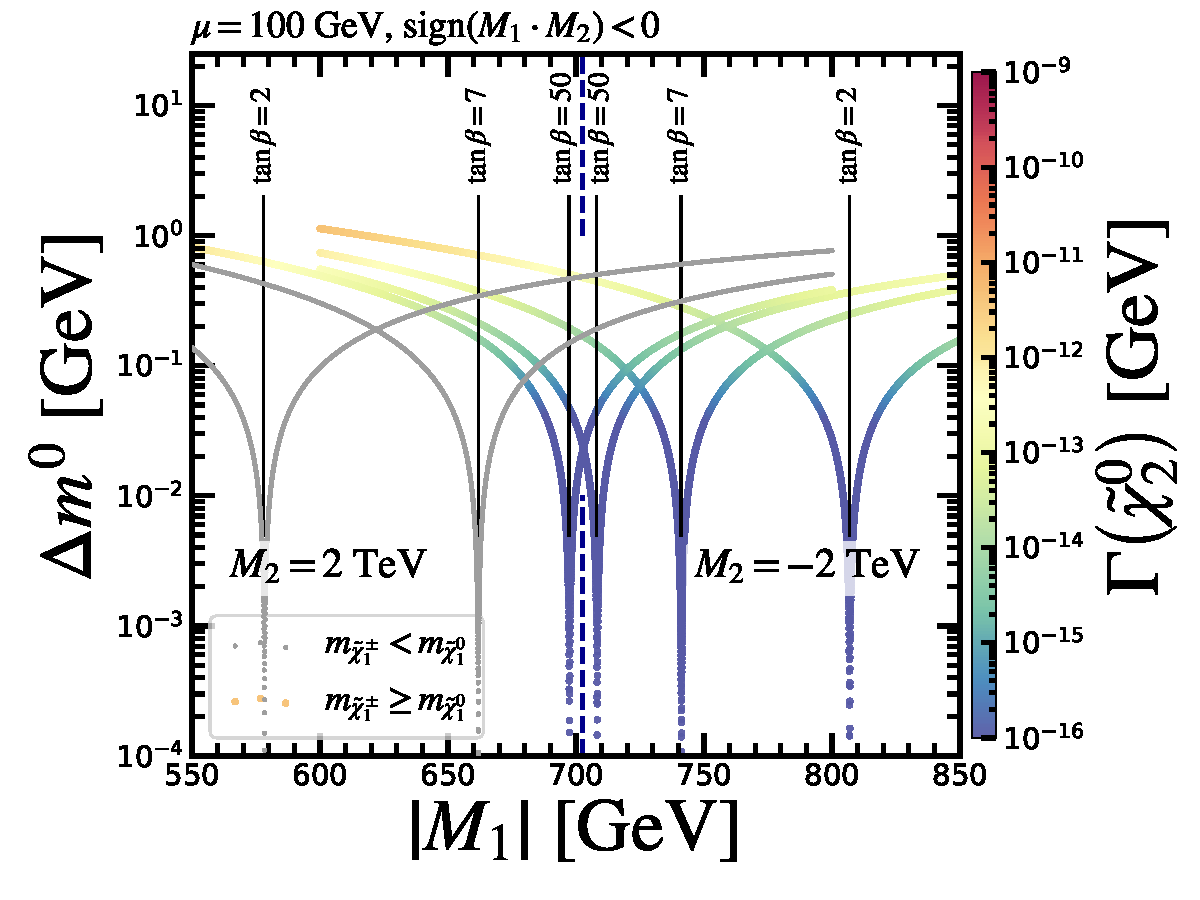
\includegraphics[width=0.5\linewidth]{M1dmN.pdf}
	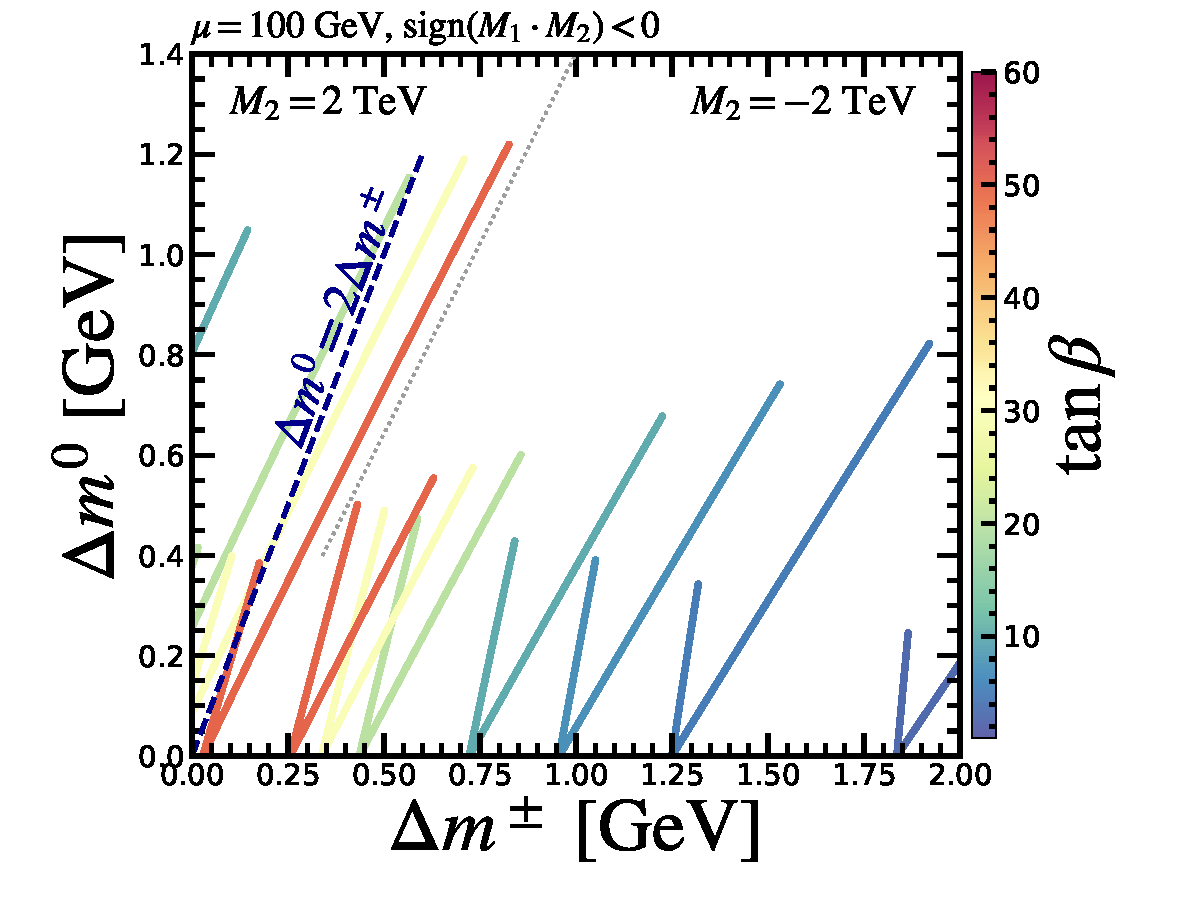
\includegraphics[width=0.5\linewidth]{dmNdmC.pdf}
    }
    \vspace{-.8cm}
	\caption{\label{fig:para} The samples in the $(\left| M_{1}\right|, \Delta m^{0})$ plane (left) and $(\Delta m^{\pm}, \Delta m^{0})$ plane (right), color-coded by $\Gamma_{\tilde{\chi}^0_2}$ (left) and $\tan\beta$ (right), respectively; grey points denote charged Higgsino LSPs.   
    % \Shufang{For the right panel, can we do a reference line of $\Delta m^0=2 \Delta m^\pm$?}
    }
\end{figure}
%%%%%%%%%%%%%%%%%%%%%%%%%%%%%%%%%%%%%%%%%%%%%%

The right panel of Fig.~\ref{fig:para} shows $\Delta m^\pm$ verses $\Delta m^0$ panel with $\tan{\beta}$ indicated by the heat map. Each broken line contains two line segments with different slopes, for $\tilde{H}_{1}^0$ or $\tilde{H}_2^0$ being the LSP, as shown in Eq.~(\ref{eq:mnue}).
The dahsed line separate the region of $M_2=\pm 2$ TeV. In the general MSSM parameter space of Higgsino LSP with $\Delta m^0 > 1~{\rm GeV}$, 
% $m_{\tilde{\chi}_1^\pm} \sim (m_{\tilde{\chi}_1^0} + m_{\tilde{\chi}_2^0})/2$ \px{
$\Delta m^0 \approx 2 \Delta m^\pm$ holds approximately, as shown in the leading terms of Eqs.~(\ref{eq:msplitn2n1}) and (\ref{eq:msplitc1N1}).   However, in the compressed regime ($\Delta m^0 < 1~{\rm GeV}$) studied in this paper, this relation no longer holds. $\Delta m^\pm$ could be in the range of a few GeV while $\Delta m^0$ remains small. This has important implication on the current experimental search limits, as explained in the next section. 


% \begin{figure}[h]
% \centering
% 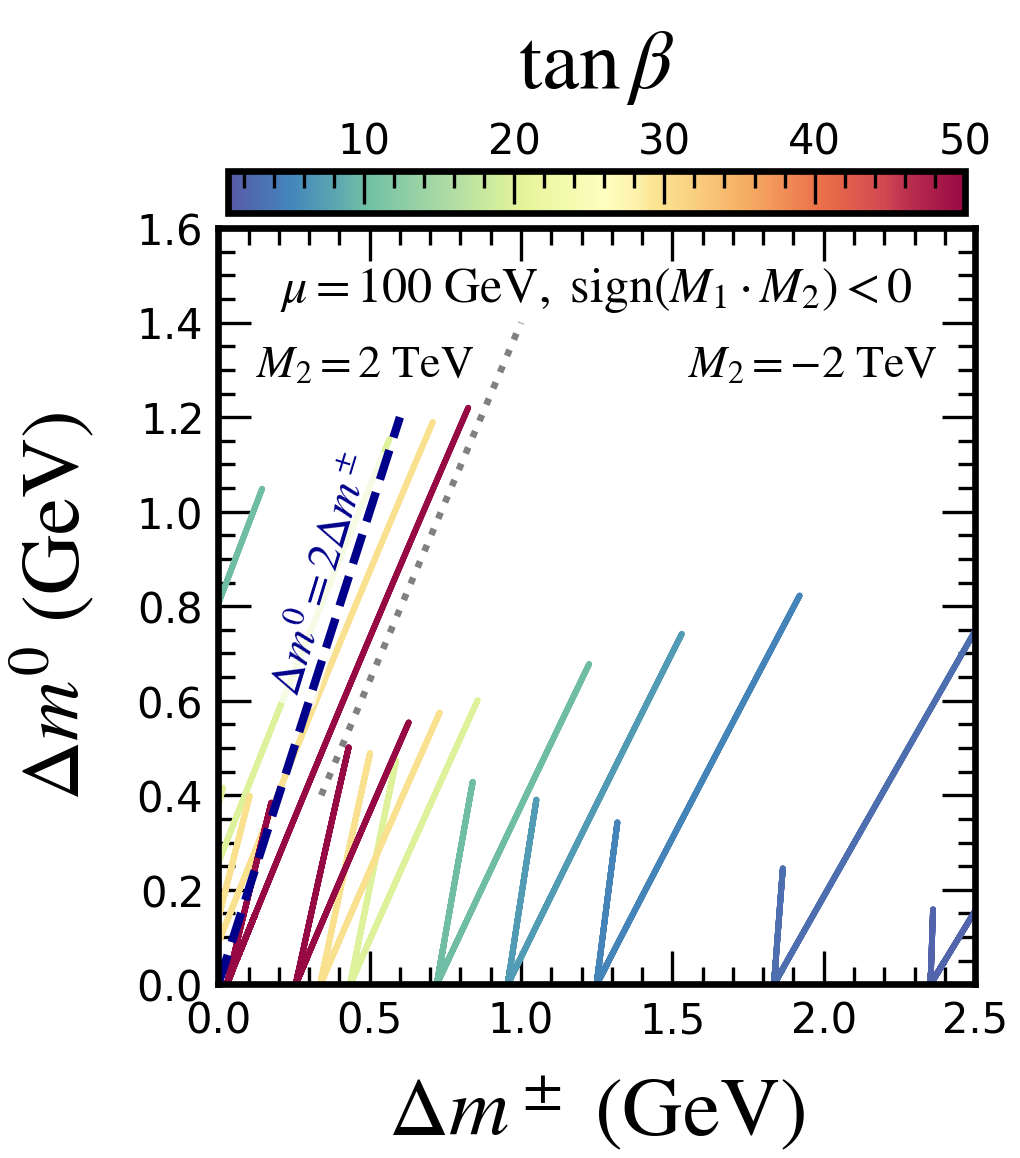
\includegraphics[width=0.6\linewidth]{dmCdmN.png}
% \vspace{-.5cm} 
% \caption{\label{fig:dcmdnm} Same samples to Fig.~\ref{fig:para}, but in $\Delta m^\pm$ verses $\Delta m^0$ panel.  }
% \end{figure}

% \Wei{here we need the $\Gamma$ to address why we need small $\Delta m^0$}
% In our case, the mass difference $\Delta m^0$ is very small. Consequently, $\tilde{\chi}_2^0$ primarily decays into $\tilde{\chi}_1^0$ and a $\gamma$, or it undergoes a three-body decay via an off-shell $Z$ boson.
% % 
% \begin{equation}
% \tilde{\chi}_2^0 \to \tilde{\chi}_1^0 + \gamma / Z^* ~~(Z^* \to f\bar{f})
% \end{equation}


% % 
% The decay of the neutralino has been investigated in Refs.~\cite{Haber:1988px, Gunion:1987yh, Ambrosanio:1995az, Ambrosanio:1996gz, Baer:2002kv}, The numerical calculations are summarized and implemented in the \texttt{SDECAY}~\cite{Djouadi:2006bz}. 
% When the mass splitting $\Delta m^0$ is less than 1 GeV, $\tilde{\chi}_2^0$ primarily undergoes radiative decay.
% \begin{equation}
% 	\Gamma(\tilde{\chi}_2^0 \to \tilde{\chi}_1^0 \gamma) = \frac{g_{\tilde{\chi}_2^0 \tilde{\chi}_1^0 \gamma}^2 }{8 \pi } \frac{\left( m_{\tilde{\chi}_2^0}^2 - m_{\tilde{\chi}_1^0}^2 \right)^3}{m_{\tilde{\chi}_2^0}^5},
% \end{equation}
% where $g_{\tilde{\chi}_2^0 \tilde{\chi}_1^0 \gamma} \propto e g^2 /16\pi^2 $  is an effective coupling arising from the one-loop diagrams.
% We have checked that for $\mu$ in the range of $100~{\rm GeV}$ to $500~{\rm GeV}$, the branching ratio of $\tilde{\chi}_2^0$ decays into $\tilde{\chi}_1^0 Z^\star$ is about $30\%$ for a mass splitting of $1~{\rm GeV}$. When the mass splitting reaches below $0.1~{\rm GeV}$, the branching ratio $\text{BR}(\tilde{\chi}_2^0 \to \tilde{\chi}_1^0 Z^\star)$ decreases to less than $1\%$. \Wei{this can be moved forward.}\Shufang{Is chi10 pi channnel important?}

% \Wei{ reduce the basic susy equtions, add more discussions along with our motivation}

% \begin{figure}[h]
% 	\centering
% 	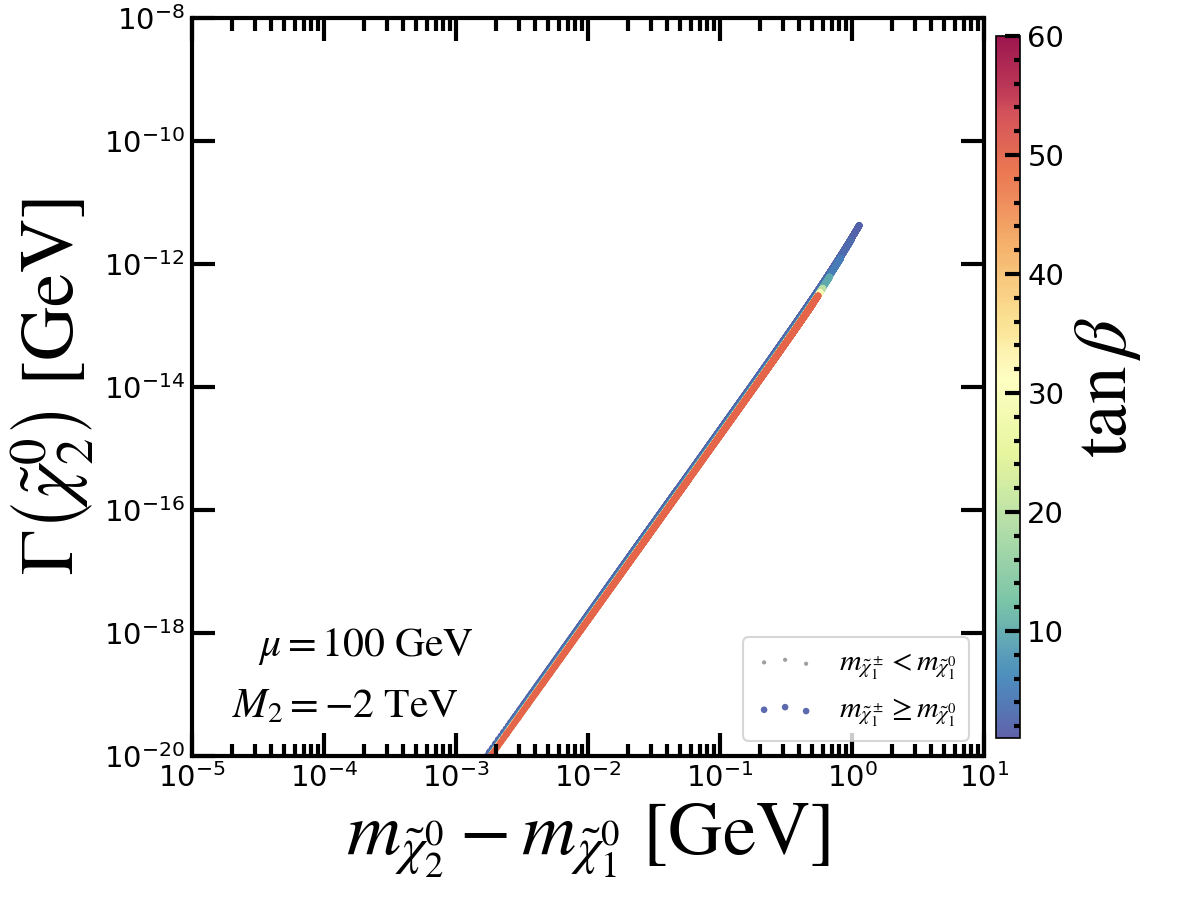
\includegraphics[width=0.48\linewidth]{dkdm100m.png}
% 	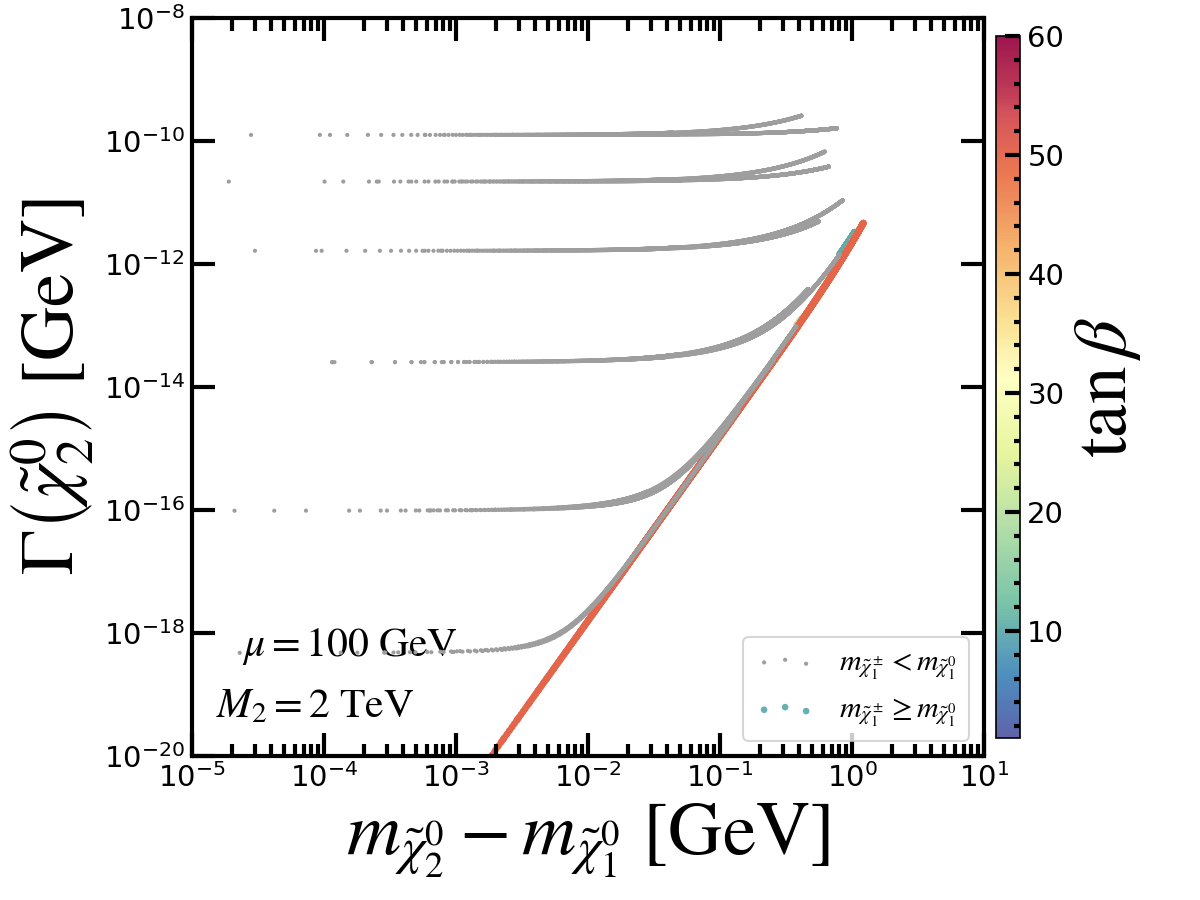
\includegraphics[width=0.48\linewidth]{dkdm100p.png}
%     \vspace{-.3cm} 
% 	\caption{\label{fig:dkdm} Same samples to Fig.~\ref{fig:para}, but in $\Gamma(\tilde{\chi}_2^0)$ verses $\Delta m^0$. The color scale indicates the value of $\tan\beta$. The blue dashed lines denote the branching ratio for the decay mode ${\rm BR}(\tilde{\chi}_2^0 \to  \tilde{\chi}_1^0 Z^*)$.  }
% \end{figure}
 

% Figure~\ref{fig:dkdm} presents the correlation between the decay width of the heavier neutralino, $\Gamma\left(\tilde{\chi}_2^0\right)$, and the mass splitting $\Delta m^0$, using the same samples set as in Fig.~\ref{fig:para}. As seen in the plot, there is an obvious power-law relationship between the decay width and the mass splitting. The effect of $\tan\beta$ on this power law relationship is negligible. 

\begin{figure}[t]
	\centering
	
\includegraphics[width=\linewidth]{notes_template/exp_constrain.png}
    \vspace{-.8cm}
\caption{\label{fig:expconstrain} 
Experimental constraints on nearly pure Higgsino electroweakinos in the plane of mass splittings versus the neutralino (left) and chargino (right) masses.  Projected sensitivities from FASER~2 are shown for $\tan\beta = 2$ (solid) and $\tan\beta = 50$ (dashed) in the left panel. 
% \Shufang{Remove references in the legend.}
}
\end{figure}
%%%%%%%%%%%%%%%%%%%%%%%%%%%%%%%%%%%%%%%%%%%%%%

%%%%%%%%%%%%%% section Constraints %%%%%%%%%%%%%%%%%
\vspace{0.5em}\noindent
\textbf{Experimental Constraints.}
\label{sec:exp}
%%%%%%%%%%%%%%%%%%%%%%%%%%%%%%%%%%%%%%%%%%%%%%
% 
%%%%%%%%%%%%%% Figure 2 %%%%%%%%%%%%%%%%%
Extensive searches at LEP and the LHC constrain the Higgsino sector. Figure~\ref{fig:expconstrain} shows the corresponding 95\% C.L. exclusion contours in the neutralino and chargino mass splitting planes.
% Searches at the LEP analyzed the chargino pair production with $\Delta m^\pm$ around xxx GeV (gray)~\cite{Abdallah:2002aik, DELPHI:1999jsl, ALEPH:2002gap, L3:1999twz, DELPHI:1997tcq}. \Shufang{displaced vertex? soft products? }  Searches for $\chi_2^0$ with $\Delta m^0 \lesssim 1~{\rm GeV}$, but the detection ability is even weaker~\cite{DELPHI:2000ijd}. 
LEP chargino searches probed $\tilde{\chi}^+_1\tilde{\chi}^-_1$ production across a broad range of mass splittings $\Delta m^\pm$, using ISR-photon tagging with soft decay products, and displaced or quasi-stable tracks in the most compressed regime (gray region)~\cite{Abdallah:2002aik,DELPHI:1999jsl,ALEPH:2002gap,L3:1999twz,DELPHI:1997tcq}.
% \Shufang{What's the limit? Is this paper relevant?} \px{LEP constraint only relate to $\Delta m^\pm$, not $\Delta m^0$.}
Both ATLAS and CMS has conducted searches of nearly degenerate Higgsinos in various channels. These include multilepton final states with missing transverse momentum~\cite{ATLAS:2021moa, ATLAS:2019lng, CMS:2021edw}, monojet signatures (red)~\cite{ATLAS:2020syg, ATLAS:2021kxv, Buanes:2022wgm, CMS:2021far, Agin:2023yoq},
compressed electroweakino searches (cyan)~\cite{CMS-PAS-EXO-23-017}), and ISR-assisted production (pink) for electroweakino in highly compressed mass spectra~\cite{ATLAS:2024woy}. 
Constraints specific to charginos include low-momentum mildly displaced vertex track searches (green)~\cite{ATLAS:2024umc, CMS:2025twk} and disappearing track searches (orange)~\cite{ATLAS:2022rme, CMS:2023mny}).   

% for squarks on jets plus $E_{\rm T}^{\rm miss}$ signature~\cite{ATLAS:2020syg, ATLAS:2021kxv}. \px{This two is the ATLAS jets + MET searches, which are recasted by Ref.~\cite{Buanes:2022wgm} for Higgsino signals. They are shown in Fig. 2, namely the monojet searches. }
% 
% Similarly about the CMS detector, we find the relevant reports including search for general SUSY compressed mass spectrum~\cite{CMS-PAS-SUS-23-003}\cite{CMS:2025ttk}.
% \Shufang{Do these two bounds appear in the Fig. 2?}
% \px{Update the bibtex of \cite{CMS-PAS-SUS-23-003}, I check the report, CMS using the assumption Delta m0 = Delta m+, and set a lower bound on Delta m+ of 3 GeV, so it is irrelavent to our work. But I can update Fig. 2}
The left panel shows that current LHC searches for nearly degenerate $\tilde{\chi}^0_2$ states lose sensitivity for $\Delta m^0 \lesssim 1~\rm{GeV}$. 
Existing neutralino limits typically assume the relation $\Delta m^0 = 2 \Delta m^\pm$, which does not hold in the small $\Delta m^0$ region relevant here; the neutralino bounds are therefore conservative when this relation is relaxed. 

In this work, $\Delta m^0$ and $\Delta m^\pm$ are allowed to vary independently, as is generically possible in the Higgsino spectrum once the gaugino masses are not tied to a fixed relation.
Consequently, for an experimental constraint appearing in both panels of Fig.~\ref{fig:expconstrain}, a parameter point is excluded only 
if the neutralino and chargino conditions are simultaneously satisfied. 
% \Shufang{Does the strong exclusion of the chargino impact the neutralino mass limits? Comment on the purple and blue limits in the right panel. } \px{Solved.}



% 

% 
%
% \begin{table*}[t]
% \centering
% \renewcommand{\arraystretch}{1.2}
% \resizebox{\linewidth}{!}{
% \begin{tabular}{llllll}
% \toprule
% \multirow{2}{*}{\textbf{Analysis/Experiment}} 
%   & \multicolumn{2}{c}{\textbf{Mass Splitting Sensitivity}} 
%   & \multirow{2}{*}{\textbf{Production Mode}} 
%   & \multicolumn{2}{c}{\textbf{Decay Mode}} 
%  \\
% \cmidrule(lr){2-3} \cmidrule(lr){5-6}
%   & $\Delta m(\tilde{\chi}_1^\pm,\,\tilde{\chi}_1^0)~[{\rm GeV}]$ 
%   & $\Delta m(\tilde{\chi}_2^0,\,\tilde{\chi}_1^0)~[{\rm GeV}]$ 
%   & 
%   & $\tilde{\chi}_1^\pm$ 
%   & $\tilde{\chi}_2^0$ 
%  \\
% \midrule
% LEP2 $\tilde{\chi}_1^\pm$ exclusion~\cite{Abdallah:2002aik, DELPHI:1999jsl, ALEPH:2002gap, L3:1999twz, DELPHI:1997tcq} 
%   & $> 0$ & -- 
%   & $e^+e^- \to \tilde{\chi}_1^+ \tilde{\chi}_1^- (\gamma)$  
%   & $W^{(\star)} \tilde{\chi}_1^0$ 
%   & -- 
% \\
% ATLAS soft-2$\ell$ or 3$\ell$~\cite{ATLAS:2021moa, ATLAS:2019lng}
%   & $> 1.5$  & $> 3$ 
%   & $\tilde{\chi}_1^\pm \tilde{\chi}_2^0 / \tilde{\chi}_1^0 \tilde{\chi}_2^0 /\tilde{\chi}_1^+ \tilde{\chi}_1^-$ 
%   & $W^{(\star)}\tilde{\chi}_1^0 $ 
%   & $Z^{(\star)} (\to \ell\ell) \tilde{\chi}_1^0 $ 
% \\
% CMS soft-2$\ell$ or 3$\ell$~\cite{CMS:2021edw}
%   & $1.5 - 10$ & $3 - 20$ 
%   & $\tilde{\chi}_1^\pm \tilde{\chi}_2^0 / \tilde{\chi}_1^0 \tilde{\chi}_2^0 $ 
%   & $W^{(\star)} (\to \ell \nu)\tilde{\chi}_1^0 $ 
%   & $Z^{(\star)} (\to \ell\ell) \tilde{\chi}_1^0 $ 
% \\
% ATLAS monojet~\cite{ATLAS:2021kxv, Buanes:2022wgm}
% & $0.5 - 1.5 $	& $1 - 3$
% & $(\tilde{\chi}_1^\pm \tilde{\chi}_2^0  /   \tilde{\chi}_1^\pm \tilde{\chi}_1^0  /  \tilde{\chi}_1^+ \tilde{\chi}_1^-) + {\rm jets}$
% & -- & -- 
% \\
% CMS monojet~\cite{CMS:2021far, Agin:2023yoq}
% & $0.45 - 2.5 $	& $0.9 - 5$
% & $(\tilde{\chi}_1^\pm \tilde{\chi}_2^0  /   \tilde{\chi}_1^\pm \tilde{\chi}_1^0  /  \tilde{\chi}_1^+ \tilde{\chi}_1^-) + {\rm jets}$
% & -- & -- 
% \\  
% CMS compressed EWino~\cite{CMS-PAS-EXO-23-017}
%   & $0.5 - 12 $ & $1 - 25$
%   & $\tilde{\chi}_1^\pm \tilde{\chi}_2^0$ + ISR 
%   & $W \tilde{\chi}_1^0 $ 
%   & $Z \tilde{\chi}_1^0 $ 
% \\
% ATLAS displaced track~\cite{ATLAS:2024umc}  
%   & $0.3 - 0.8$ & --
%   & $\tilde{\chi}_1^\pm \tilde{\chi}_{1/2}^0 / \tilde{\chi}_1^+ \tilde{\chi}_1^-$ 
%   & a several cm track
%   & --  
% \\
% CMS displaced track~\cite{CMS:2025twk}
% & $0.3 - 1.0$ 	& -- 
% & $\tilde{\chi}_1^\pm \tilde{\chi}_{1/2}^0 / \tilde{\chi}_1^+ \tilde{\chi}_1^-$
% & a several cm track	&	-- 
% \\
% ATLAS disappearing-track~\cite{ATLAS:2022rme} 
%   & $< 0.3$  & --
%   & $pp \to \tilde{\chi}_1^\pm \tilde{\chi}_{1/2}^0 / \tilde{\chi}_1^+ \tilde{\chi}_1^- $ + jets 
%   & long-lived $\tilde{\chi}_1^\pm$ 
%   & -- 
% \\
% CMS disappearing track~\cite{CMS:2023mny}
%  & $< 0.36 $	& -- 
%  & $pp \to \tilde{\chi}_1^\pm \tilde{\chi}_{1/2}^0 / \tilde{\chi}_1^+ \tilde{\chi}_1^- $ + jets 
%  & long-lived $\tilde{\chi}_1^\pm $	& -- 
%   \\
% ATLAS EWino di-jet~\cite{ATLAS:2024woy}
%   & -- & --  & $\tilde{\chi}_1^\pm \tilde{\chi}_2^0$ + 2 ISR 
%   & -- & --
% \\
% \bottomrule
% \end{tabular}
% }
% \caption{\label{tab:exp} Summary of for Higgsino searches at LEP and the LHC. The mass splitting sensitivity ranges correspond to the regions probed by each analysis for a Higgsino mass of 100~GeV. \px{Remove this tables}
% }
% \label{tab:Higgsino_masssplitting}
% \end{table*}
% 
% 
%
% , and the corresponding simplified model are summarized in Table.~\ref{tab:exp}, focusing on the mass splitting intervals explored for a Higgsino mass of 100~GeV.


%%%%%%%%%%%%%% Figure 3 %%%%%%%%%%%%%%%%%

%%%%%%%%%%%%%%%%%%%%%%%%%%%%%%%%%%%%%%%%%%%%%%

%%%%%%%%%%%%%%%%%% Section FASER %%%%%%%%%%%%%%%
\vspace{0.5em}\noindent
\textbf{FASER sensitivity to LLP $\tilde{\chi}_2^0$.}
\label{sec:faser}
% 
%%%%%%%%%%%%%%%%%% Overview %%%%%%%%%%%%%%%%%%%%
% \Wei{this section could have more discussions.}
% The FASER~\cite{Feng:2022inv, FASER:2018eoc} experiment is designed to search for long lived particle at the LHC forward region.  The detector is located in a service tunnel 480 m downstream of the ATLAS interaction point (IP), precisely on the beam collision axis.   The detector is a compact cylindrical aligned with the beam axis, with the radius $R = 0.1~{\rm m}$ and length $D=1.5~{\rm m}$ for an integrated luminosity $150~{\rm fb}^{-1}$. For the FASER 2 at the future HL-LHC, it will be updated to $R = 1~{\rm m}$ and length $D=5~{\rm m}$ for a integrated luminosity of $3~{\rm ab}^{-1}$. \Shufang{Does the location change?} 
% \px{I think you said FASER 2 is locate in 620 m of the IP.}


The FASER experiment~\cite{Feng:2022inv, FASER:2018eoc} is designed to search for long-lived particles produced in the far-forward region at the LHC. 
It is located in a service tunnel approximately $480~\mathrm{m}$ downstream of the ATLAS interaction point (IP), aligned with the beam collision axis. 
The detector consists of a compact cylindrical decay volume with radius $R = 0.1~\mathrm{m}$ and length $D = 1.5~\mathrm{m}$, corresponding to an integrated luminosity of $150~\mathrm{fb}^{-1}$.  

At the HL-LHC, FASER~2 is expected to operate at $L=620~\mathrm{m}$ with a cylindrical decay volume of $R=1~\mathrm{m}$ and $D=10~\mathrm{m}$, corresponding to an integrated luminosity of $3~\mathrm{ab}^{-1}$.%
\footnote{Several design configurations for FASER~2 have been discussed in the literature\px{May need some Refs.}. In this work, we adopt a representative benchmark geometry for concreteness. We have verified that moderate variations of the detector dimensions within the proposed design range do not qualitatively affect the sensitivity of FASER~2 to compressed Higgsino scenarios.}
% Key detector parameters for FASER and its proposed FASER 2 upgrade can be summarised as:
% \begin{equation}\begin{split}
% 	&\text{FASER}: \quad 
% 	R = 0.1~{\rm m}, \quad
% 	D = 1.5~{\rm m},\quad
% 	\mathcal{L}_{\rm int} = 150~{\rm fb}^{-1};  \\
% 	&\text{FASER 2}: \quad 
% 	R = 1~{\rm m}, \quad 
% 	D = 5.0~{\rm m}, \quad
% 	\mathcal{L}_{\rm int} = 3~{\rm ab}^{-1},
% \end{split}\end{equation}
% where $R$ and $D$ are the radius and length of the detector cylinder.   
% % % 
% \par FASER and FASER 2 are designed to efficiently reconstruct LLPs whose decay products—such as electrons, muons, photons, and hadrons—are highly collimated along the beam direction. To enhance sensitivity to photon final states, a preshower detector based on monolithic silicon pixel sensors has been proposed~\cite{Boyd:2803084}. This enables the efficient detection of photons resulting from $\tilde{\chi}_2^0$ decays.

% \par For a LLP with mass $m$ produced at the IP with momentum $p$, angle $\theta$ with respect to the beam axis and the decay width $\Gamma$, the probability that it will decay within the detector volume of FASER is
% % \begin{equation}\label{eq:Faserprob}
% % \begin{split}
% % 		{\rm Prob}({\rm FASER}) &= e^{-\frac{(L+D) m \Gamma}{p}} \left( e^{\frac{D m\Gamma}{p}} -1\right) \Theta(R-\tan{\theta}L), \\
% % 		&\approx \frac{D}{\lambda} e^{-\frac{L}{\lambda}} \Theta(R-\tan{\theta}L). 
% % \end{split} 
% % \end{equation}
% \begin{equation}\label{eq:Faserprob}
% \begin{split}
% 		{\rm Prob}({\rm FASER}) = \frac{D}{\lambda} e^{-\frac{L}{\lambda}} \Theta(R-\tan{\theta}L). 
% \end{split} 
% \end{equation}
% Here, $\Theta(x)$ denotes the Heaviside step function, and the characteristic decay length $\lambda$ of the LLP in the laboratory frame is
% \begin{equation}
% 	\lambda = c \tau \beta \gamma  = \frac{p}{m\Gamma},
% \end{equation}
% where $\tau=1/\Gamma$ is the proper lifetime (with total width $\Gamma$), and $\beta=v/c$ and $\gamma=1/\sqrt{1-\beta^2}$ are the usual Lorentz factors.
For a LLP of mass $m$ and decay width $\Gamma$, produced at the IP with momentum $p$ and polar angle $\theta$, the probability to decay inside the fiducial volume of FASER or FASER~2 is approximately
\begin{equation}\label{eq:FASERprob}
    \mathrm{Prob}_{\rm FASER} \simeq \frac{D}{\lambda} e^{-L/\lambda} \Theta \left(R - L\tan\theta\right),
\end{equation}
where  
$ \lambda = \frac{p}{m\,\Gamma} = c\tau\,\beta\gamma $
is the mean LLP decay length in the lab frame, $\tau = 1/\Gamma$ its proper lifetime, and $\Theta(x)$ the Heaviside step function enforcing the condition that the particle’s trajectory enters the detector (transverse radius $R$ at a distance $L$ downstream) before decaying.

\begin{figure}
     \centering
     % 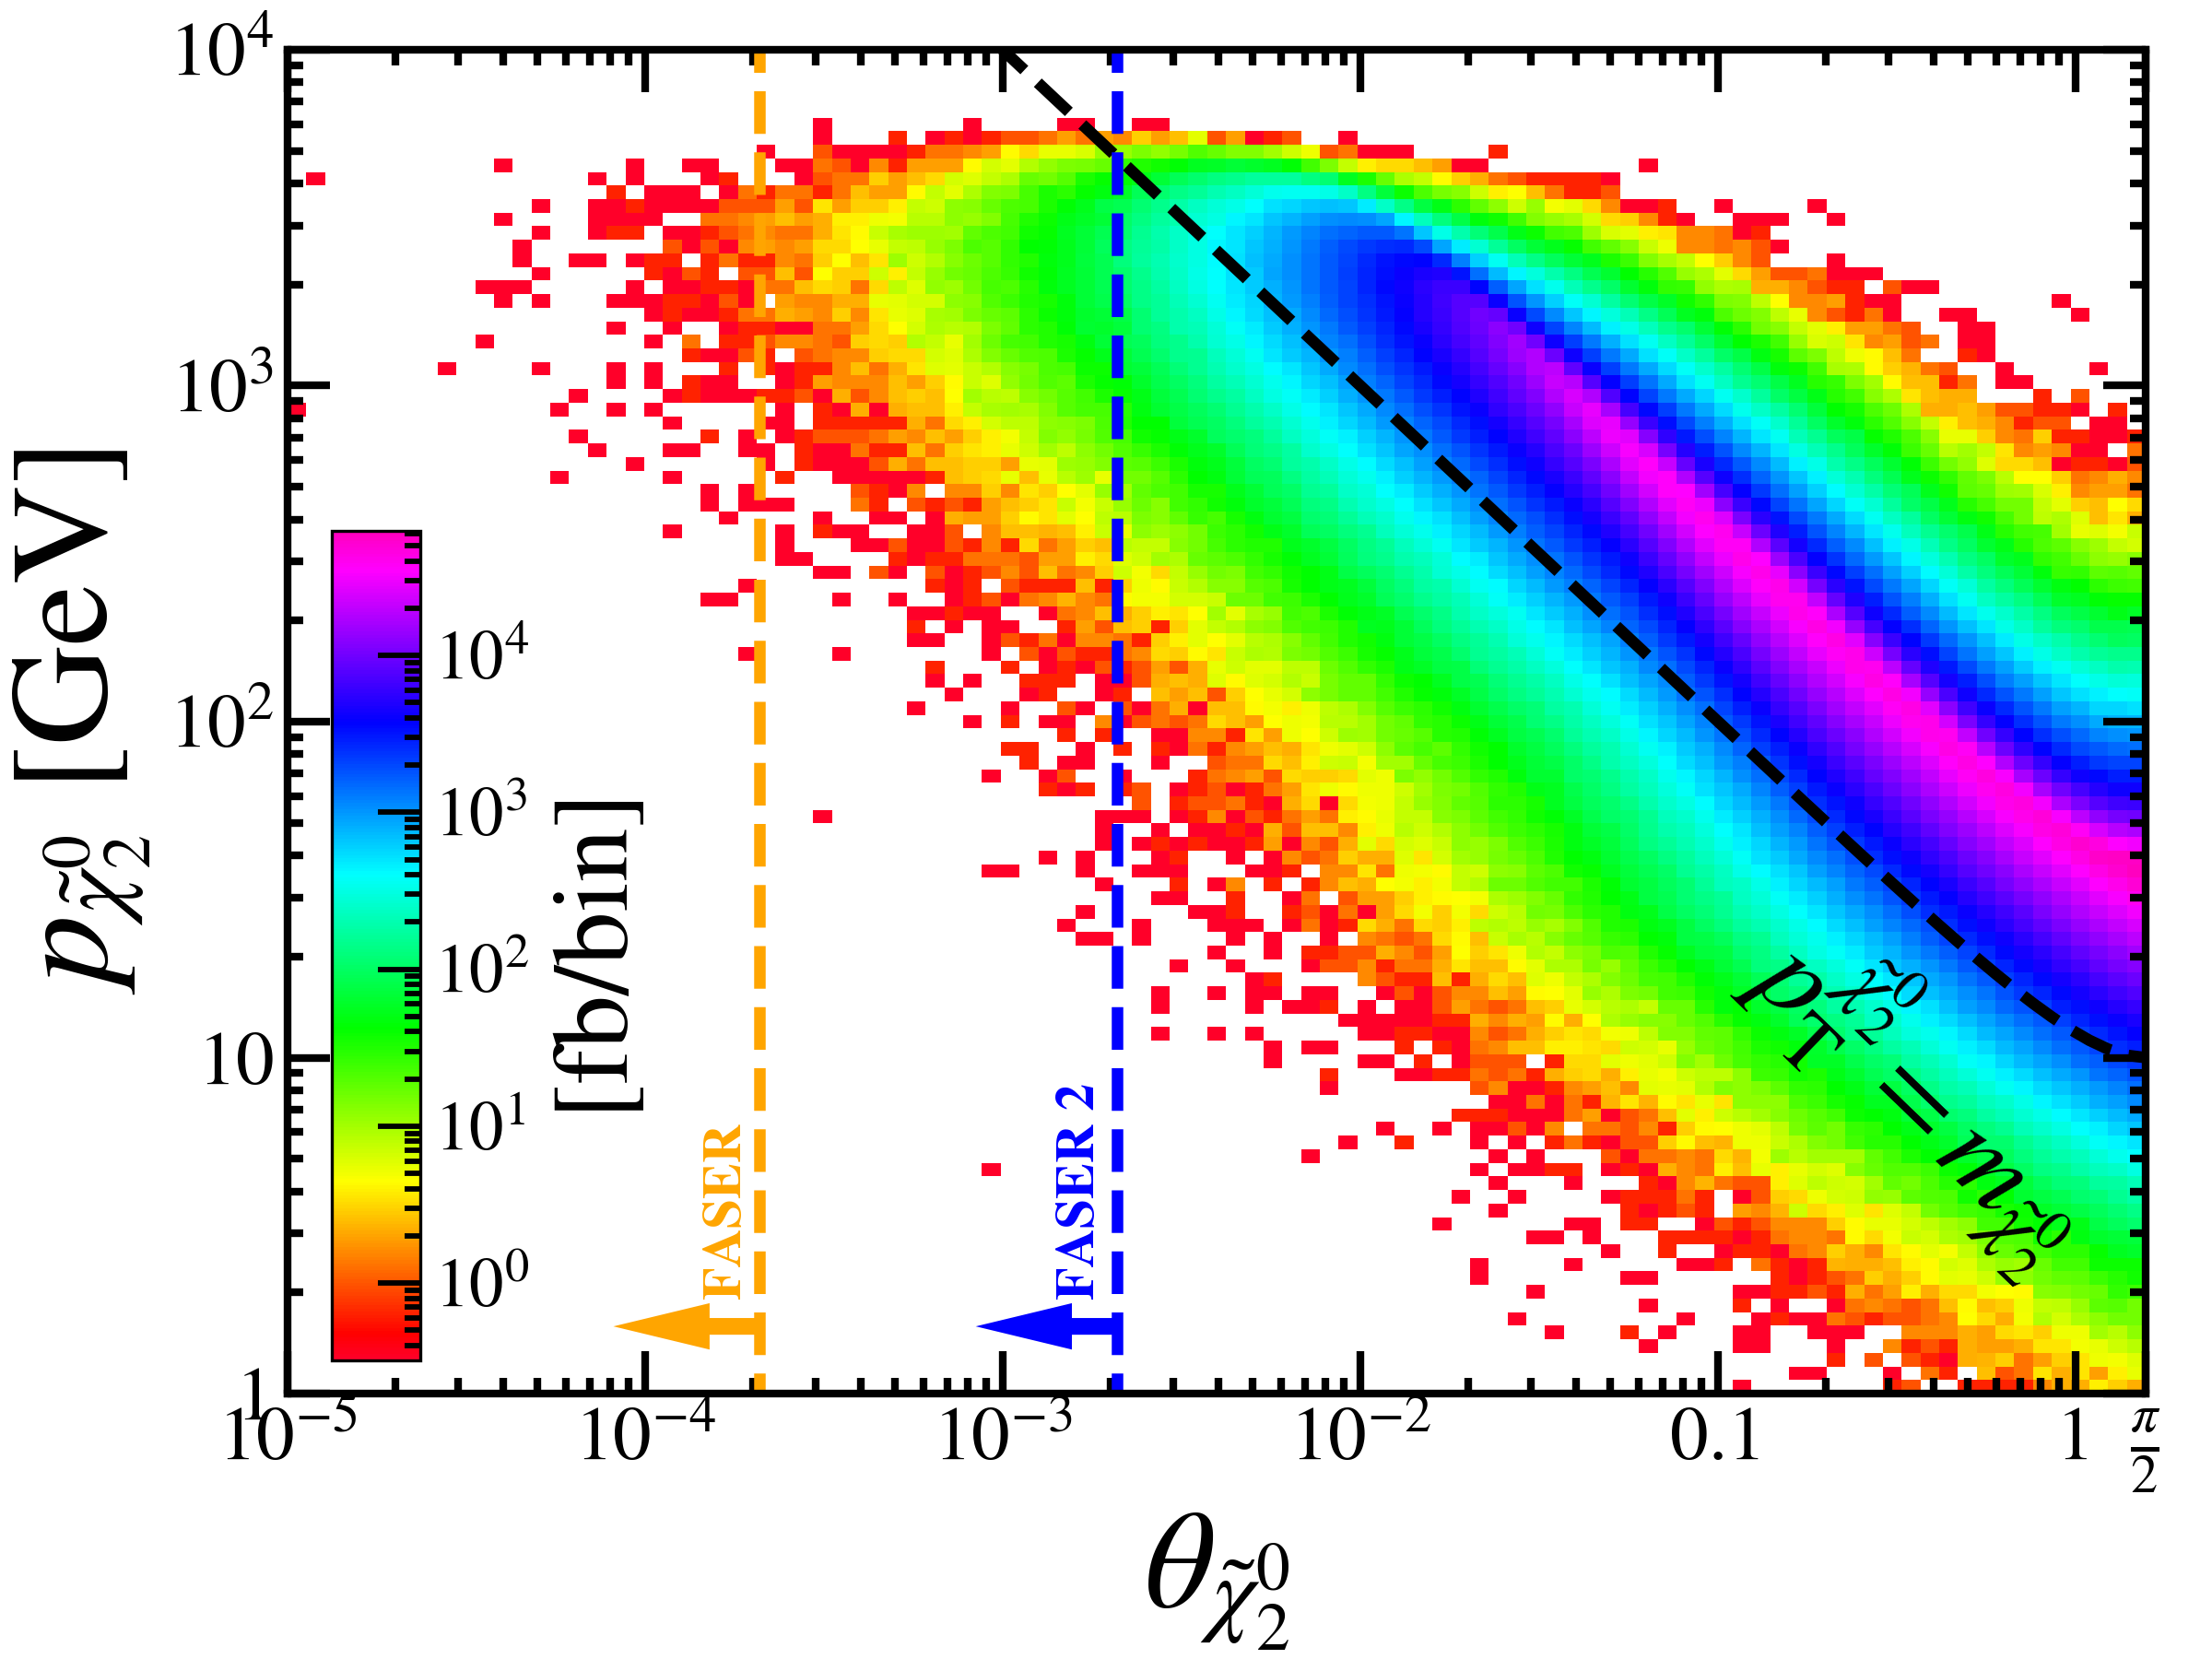
\includegraphics[width=0.48\linewidth]{10-distri.png}
     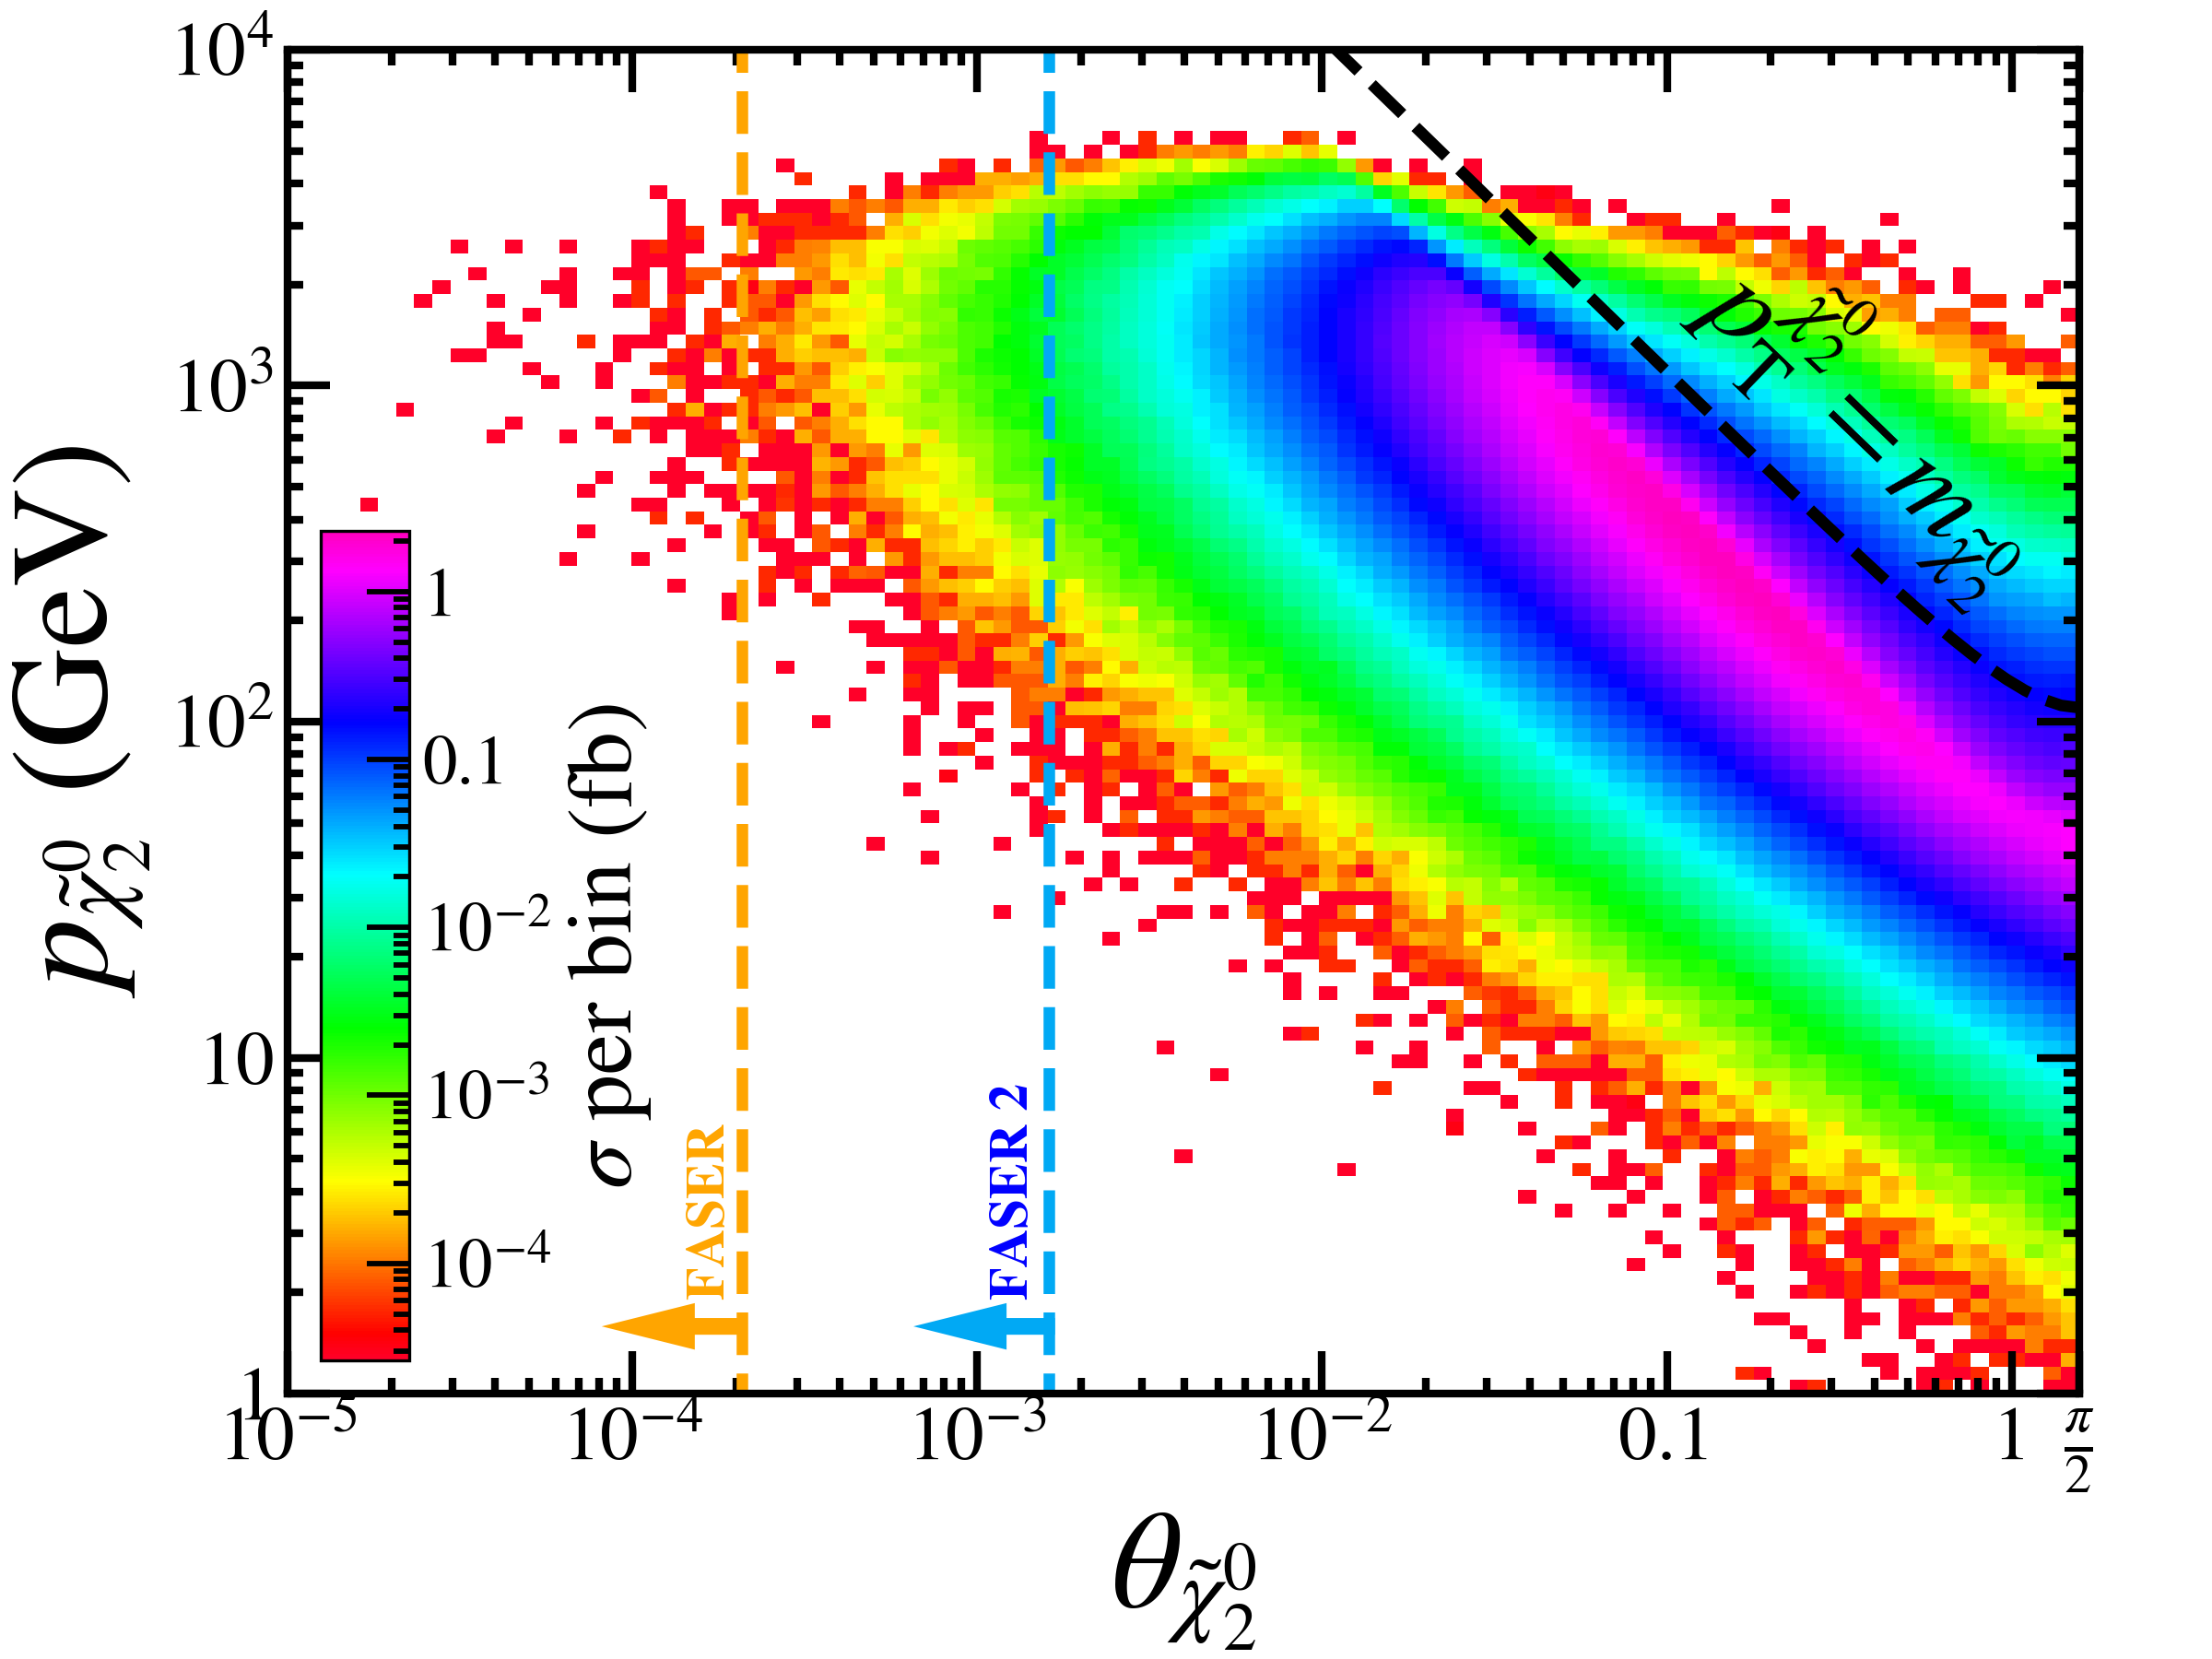
\includegraphics[width=0.75\linewidth]{110-distri.png}
     \vspace{-.3cm}
 \caption{\label{fig:xsect} 
 Density map of $p_{\tilde{\chi}_2^0}$ versus $\theta_{\tilde{\chi}_2^0}$ for $\tilde{\chi}_2^0$ production at the LHC, shown for $\mu = 110~\mathrm{GeV}$. 
The color scale represents the differential cross section per bin in unit of fb. 
Vertical dashed lines indicate the angular acceptances of FASER (orange) and FASER~2 (blue), and the black dashed curve shows $p^{\tilde{\chi}_2^0}_{\rm T} = m_{\tilde{\chi}_2^0}$.
 % \Shufang{what's the binning? only show one plot? mu=10 GeV would have been excluded already at LEP.} \px{Yes, I think we should just plot with mu = 110 GeV}
 }
\end{figure}

Typical benchmark scenarios considered in the FASER study~\cite{FASER:2018eoc} involve light long-lived particles originating from meson decays in the forward region. 
In contrast, the compressed Higgsino scenario examined here is characterized by an electroweak hard-production mechanism, proceeding through $s$-channel $Z$- or $W$-boson exchange~\cite{Haber:1984rc}.  
For the numerical analysis, we generate all Higgsino pair–production channels using \texttt{Pythia8.3}~\cite{Bierlich:2022pfr} with the Monash tune~\cite{Skands:2014pea}. 
As shown in Fig.~\ref{fig:xsect}, the produced $\tilde{\chi}_2^0$ states are highly boosted and strongly forward-peaked, with the cross section concentrated at small polar angles. 
Because FASER covers only an extremely narrow angular region, its geometric acceptance for Higgsino production is negligible. 
In contrast, the larger transverse size of FASER~2 allows substantial overlap with the forward Higgsino flux, as illustrated by the $(\theta,p)$ distribution in Fig.~\ref{fig:xsect} for the benchmark point $\mu = 110~\mathrm{GeV}$, where contributions from all production channels are included.  
The vertical dashed lines indicate the angular coverage of FASER (orange) and FASER~2 (blue), showing that only FASER~2 intercepts a significant fraction of the forward Higgsinos, whose momenta typically range from a few hundred GeV to multi-TeV values.  
The decay probability of $\tilde{\chi}_2^0$ inside the FASER or FASER~2 decay volume is evaluated using Eq.~(\ref{eq:FASERprob}).

The expected 3 event FASER 2 detection reach of a long-lived neutralino $\tilde{\chi}_2^0$ was shown in Fig.~\ref{fig:expconstrain} as blue regions.  For a Higgsino mass of around 80 to 130 GeV, FASER 2 is sensitive to the mass difference $\Delta m^0$ ranges from $0.1$ to $0.5~{\rm GeV}$. 
The FASER 2 reach has little dependence on the value of $\tan\beta$, as indicated by the blue solid (dashed) curve for $\tan\beta=2$ (50).

\begin{figure}[t]
\centering
    \makebox[\linewidth][c]{
	\hspace{-0.3cm}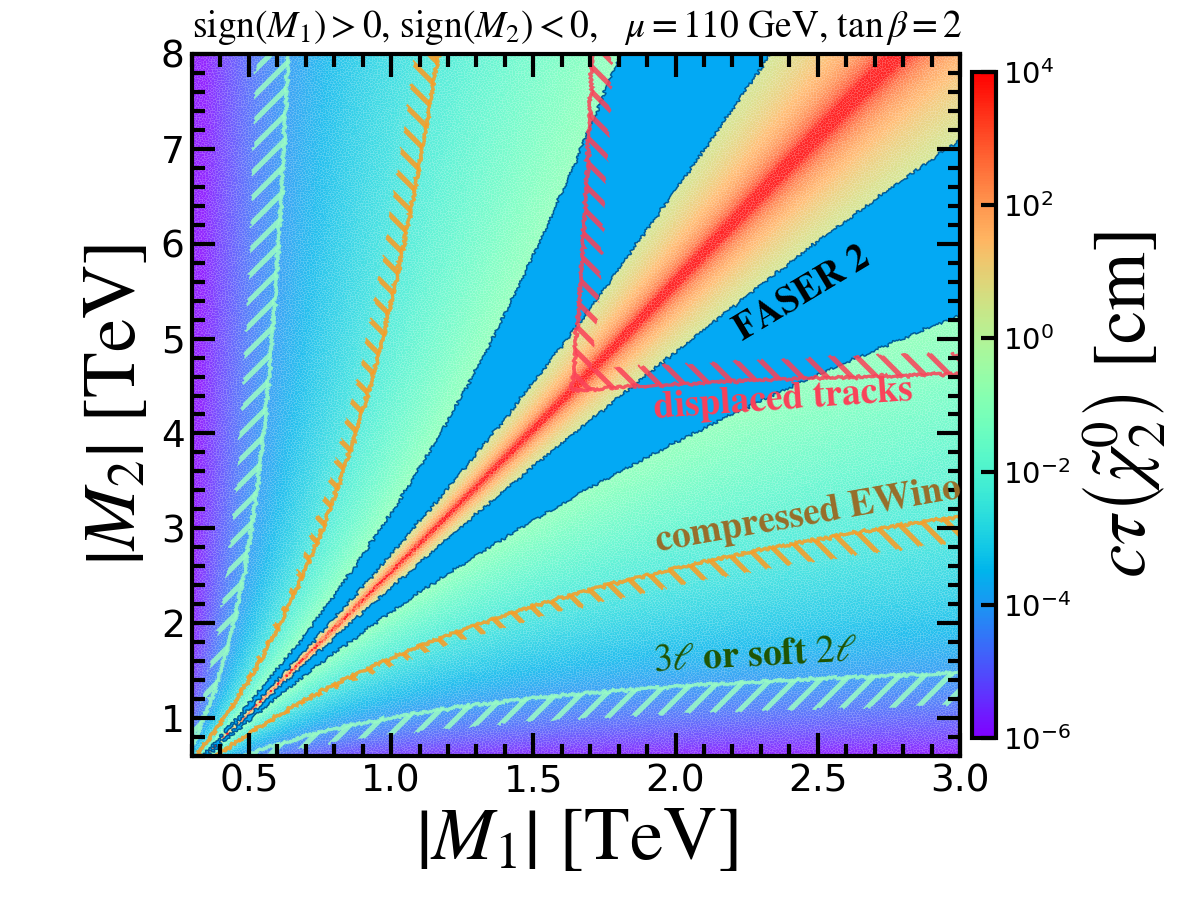
\includegraphics[width=0.52\linewidth]{mu110_TB02_M2minus.png}	
    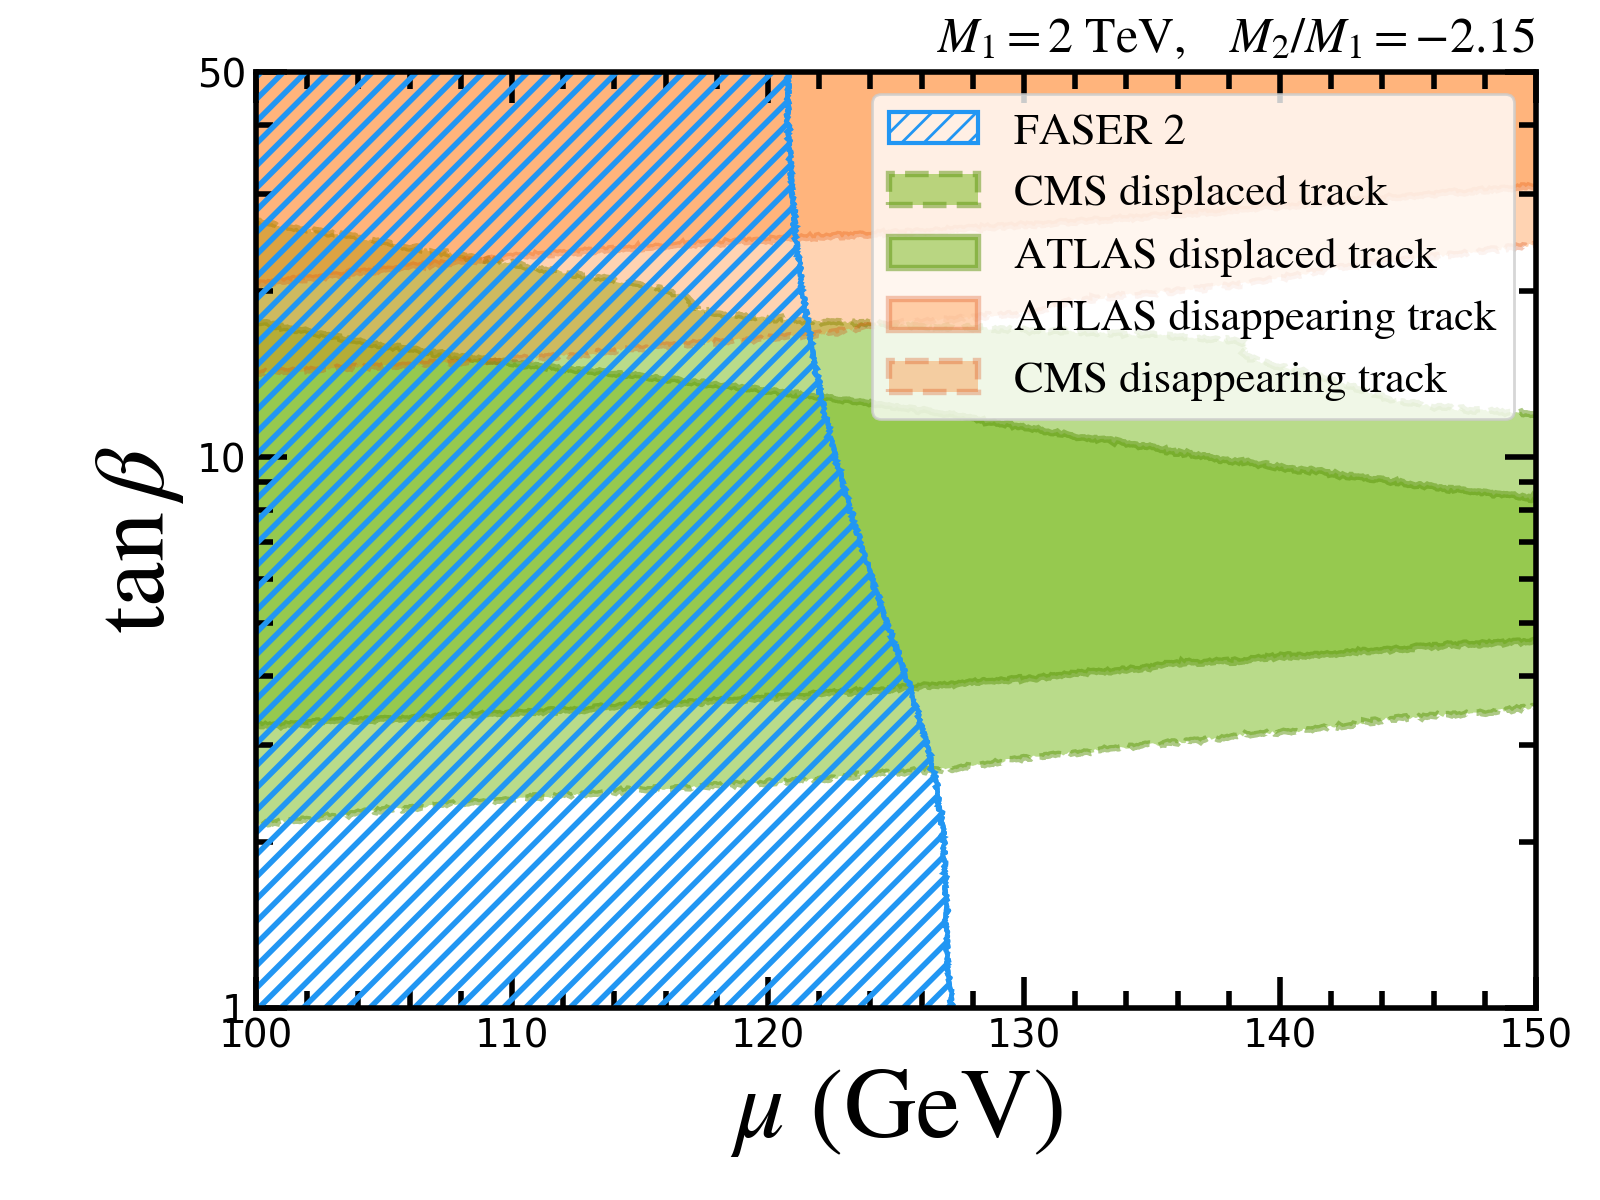
\includegraphics[width=0.52\linewidth]{muTB_logY.png}\hspace{-0.3cm}
    }
    \vspace{-.8cm}
\caption{\label{fig:ps} \textit{Left}: Coverage of LHC searches and FASER 2 in the $(|M_1|,|M_2|)$ plane, with color shading indicating the proper lifetime of $\tilde{\chi}_2^0$. \textit{Right}: Projected sensitivity of the LHC and FASER 2 in the $(\mu, \tan\beta)$ plane. 
% \Wei{update the plot}
}
\end{figure}


% Given the dependence of $\Delta m^0$ and $\Delta m^\pm$ on the MSSM mass parameters $M_1$ and $M_2$, in the left panel of Fig.~\ref{fig:ps}, we present the current LHC search coverage and the projected sensitivity of FASER 2 in $|M_1|$ versus $|M_2|$ plane with $\mu = 110~{\rm GeV}$. Conventional LHC searches, including those based on soft-lepton signatures, displaced tracks,  and disappearing tracks are illustrated with their respective exclusion regions. \Shufang{Which one is disappearing tracks? Why compressed EWino is sensitive to large Delta M? What signal is compressed EWino?} These analyses become less sensitive when the mass difference $\Delta m^0$ is small, while $\Delta m^\pm$ is significantly larger. \Shufang{which curves are you refering to? Disappearing tracks are senstivie to a range of $\Delta m^\pm$ while it is shown here for the entire region of M1, M2 larger than certain value.}  When $ M_{1,2} $ is significantly large, the chargino becomes long-lived due to the small $\Delta m^\pm$, leading to the exclusion of the top right corner of the $M_1$ vs. $M_2$ parameter space. For $\mu = 110~{\rm GeV}$, FASER 2 is sensitive to $\Gamma_{\tilde{\chi}_2^0}$ in the region of $8.8\times 10^{-15}~{\rm GeV}$ to $1.5\times 10^{-13}~{\rm GeV}$, which is shown as two bands in the $M_1-M_2$ plane, corresponding to the ratio of $M_2/M_1$ approximately within the interval $[-4.3, -3.4]$ and $[-2.3, -1.8]$.  In parameter space with a small $\tan{\beta}$ and ${\rm sign}(\mu M_2) < 0$, a large mass splitting between the chargino and the LSP is predicted. \Shufang{??? It explains why in the right plot, there is no limit in small TB for the LHC searches.}

Given the dependence of the neutralino and chargino mass splittings, $\Delta m^0$ and $\Delta m^\pm$, on the MSSM gaugino mass parameters $M_1$ and $M_2$, the left panel of Fig.~\ref{fig:ps} shows the current LHC search coverage together with the projected sensitivity of FASER~2 in the $(|M_1|,|M_2|)$ plane for a benchmark $\mu = 110~\mathrm{GeV}$. 
The shaded regions indicate exclusions from different classes of LHC searches targeting electroweakinos, including soft-lepton and multilepton searches~\cite{ATLAS:2021moa, ATLAS:2019lng, CMS:2021edw}, compressed electroweakino search~\cite{CMS-PAS-EXO-23-017}, displaced-track searches for intermediate lifetimes~\cite{ATLAS:2024umc, CMS:2025twk}, and disappearing-track searches sensitive to long-lived charginos~\cite{ATLAS:2022rme, CMS:2023mny}.

In the region of large $|M_1|$ and $|M_2|$, the chargino–LSP mass splitting $\Delta m^\pm$ becomes small, rendering the chargino long-lived. 
This behavior follows directly from Eq.~(\ref{eq:msplitc1N1}), where the leading corrections to $\Delta m^\pm$ scale inversely with the gaugino mass parameters $M_1$ and $M_2$. 
As a result, regions with large $|M_{1,2}|$, which correspond to long-lived charginos, are strongly excluded by disappearing-track searches in the upper-right corner of the $(|M_1|,|M_2|)$ plane. By contrast, in regions where only one of the gaugino masses, $M_1$ or $M_2$, lies at the sub-TeV scale, the contributions from $M_1$ and $M_2$ to the mass splittings no longer cancel. 
In this case, the spectrum reverts to the generic hierarchy $\Delta m^0 \simeq 2\,\Delta m^\pm$, leading to prompt decays of both neutralinos and charginos. 
As a result, traditional LHC searches based on multi-lepton signatures and compressed electroweakino analyses regain strong sensitivity and impose stringent constraints in this region of the parameter space. 
In the remaining region of the parameter space, where the chargino is not long-lived while the neutralino mass splitting $\Delta m^0$ remains small, conventional LHC searches lose sensitivity. In this regime, the heavier neutralino can be long-lived and highly boosted, making FASER~2 uniquely sensitive to this otherwise unconstrained region. For $\mu = 110~\mathrm{GeV}$, FASER~2 probes $\tilde{\chi}_2^0$ decay widths in the range $\Gamma_{\tilde{\chi}_2^0}\simeq (5.9\times10^{-15} - 1.4\times10^{-13})~\mathrm{GeV}$, shown as the blue bands.
These regions correspond approximately to $M_2/M_1 \in [-4.3,-3.4]$ and $[-2.3,-1.8]$, where the boosted neutralino falls within the sensitive decay volume of FASER~2.

The right panel of Fig.~\ref{fig:ps} further illustrates the projected sensitivity in the $(\mu,\tan\beta)$ plane for fixed $M_1$ and $M_2$.
For small $\tan\beta$ and ${\rm sign}(\mu M_2)<0$, when the neutralino mass splitting $\Delta m^0$ is small, the chargino–LSP mass splitting $\Delta m^\pm$ increases as $\tan\beta$ decreases, this feature can clearly seen in the right panel of Fig.~2. Therefore, displaced-track and disappearing-track searches lose sensitivity in the low $\tan{\beta}$ region. 

Overall, our analysis reveals a complementary relation between prompt LHC searches and FASER~2 in the MSSM electroweakino parameter space.
While conventional LHC analyses efficiently probe regions with sizable mass splittings or long-lived charginos, FASER~2 extends the sensitivity to scenarios with prompt charginos and small $\Delta m^0$ through displaced decays of boosted neutralinos.
Notably, the FASER~2–sensitive regions correspond to restricted ranges of the gaugino mass ratios, and a future signal would not only point to a natural SUSY spectrum but also provide valuable insight into the structure of SUSY breaking at high scales.

% \section{Conclusions}
\vspace{0.5em}\noindent
\textbf{Conclusions.}
\label{sec:sum}
\Wei{there are 2-3 works about FASER beyond 5 GeV, LLP are from H/Z decays. our production is different, does not depend on H/Z decay, and much larger mass region. Do we need to mention this?} \Shufang{Yes, we should mention those heavy particle searches at FASER.}
In our study, we investigated a particular region of the Higgsino LSP scenario ($|\mu| \ll |M_{1,2}|$) with $M_2/M_1 \approx -\tan^2{\theta_W}$, in which the Higgsino-like neutralinos $\tilde{\chi}_1^0$ and $\tilde{\chi}_2^0$ become nearly degenerate with $\Delta m^0 \lesssim 1$ GeV, resulting in a long-lived $\tilde{\chi}_2^0$. While such a scenario is challenging at the conventional LHC searches, the upcoming FASER-2 experiment offers a unique detection sensitivity. FASER 2 could cover $|\mu|$ up to about $126~{\rm GeV}$ and a mass splitting $\Delta m^0$ between 0.1 to 0.5 GeV. This corresponds to a decay width of $\Gamma_{\tilde{\chi}_2^0}$ around $ 10^{-15} - 10^{-13}~{\rm GeV}$.  There is a nice complementarity between the FASER 2 reach and the conventional LHC reach.  When combined, a significant parameter space  of the Higgsino LSP scenario can be covered.

While FASER 2 is designed to detect the long lived particle at the forward region, it is typically sensitive to light particles copiously produced via the decay of mesons.  Our study  showed that FASER~2 can also be sensitive to  particles with masses at the electroweak scale, which opens the door to explore other electroweak scale long lived new particles.

\vspace{0.5em}\noindent
\textbf{Acknowledgments.}
SS is supported by the Department of Energy under Grant No. DE-
FG02-13ER41976/DE-SC0009913. 
WS is supported by the Junior Foundation of Sun Yat-sen University and Shenzhen Science and Technology Program (Grant No. 202206193000001, 20220816094256002). 
JMY is supported by the National Natural Science Foundation of China under Grant No. 12335005 and by PI Research Fund from Henan Normal University under Grant No. 5101029470335. 
PZ is supported by the ARC Discovery Project DP220100007 and by the Center for the Subatomic Structure of Matter (CSSM).


%%%%%%%%%%%%%%%%%%%%%%%%%%%%%%%%%%%%%%%%%%%%%%

% The \nocite command causes all entries in a bibliography to be printed out
% whether or not they are actually referenced in the text. This is appropriate
% for the sample file to show the different styles of references, but authors
% most likely will not want to use it.
% \nocite{*}

\bibliographystyle{CitationStyle}
\bibliography{ref_type1}% Produces the bibliography via BibTeX.
% \bibliographystyle{unsrtnat}
% \bibliographystyle{modified-apsrev4-2.bst}
\end{document}
%
% ****** End of file apssamp.tex ******
